%       File: VTthesis_template.tex
%     Created: Thu Mar 24 11:00 AM 2016 EDT
%     Last Change: Thursday, December 19, 2019
%     Author: Alan M. Lattimer, VT
%	  With modifications by Carrie Cross, Robert Browder, and LianTze Lim. 
%
% This template is designed to operate with XeLaTeX.
%
% All elements in the Title, Abstract, and Keywords MUST be formatted as text and NOT as math.
%
%Further instructions for using this template are embedded in the document. Additionally, there are comments at the end of the file that give suggestions on writing your thesis.  
%
%In addition to the standard formatting options, the following options are defined for the VTthesis class: proposal, prelim, doublespace, draft. 

%\documentclass[doublespace,nopageskip]{VTthesis} % nopageskip - Removes arbitrary blank pages.

% Using the following header instead will create a draft copy of your thesis
\documentclass[doublespace,nopageskip]{VTthesis}
%!TeX program = xelatex
% The lipsum package is just included to put dummy text in the document in order to demonstrate page headers and table of contents behavior. You should remove it once you begin writing your actual thesis or dissertation.
%\usepackage{lipsum}

% Title of your thesis
\title{Multimodal Multi-Document Evidence Summarization For Fact-Checking
}

% You should include 3-5 keywords, separated by commas
\keywords{Knowledge Graph, Multimodal learning, Reinforcement learning and Summarization}

% Your name, including middle initial(s)
\author{Ting-Chih Chen}

% Change this to your program, e.g. Physics, Civil Engineering, etc.
\program{Computer Science and Applications} 

% Change this to your degree, e.g. Master of Science, Master of Art, etc.
\degree{Master of Science} 

% This should be your defense date:
\submitdate{December 1, 2023} 

% Committee members. Only have five readers and one chair available.
% Only use the ones you need and don't include the ones you don't need.
% You can also declare a Co-advisor. If you do, the principal and co-advisors
% will be listed as co-advisors on the title page.  Per the VT ETD standards, 
% you should not include titles or educational qualifications such as PhD or Dr.
% You should, however, include middle initials if possible.
\principaladvisor{Christopher Thomas}
\firstreader{Lifu Huang}
\secondreader{Ismini Lourentzou}


% The dedication and acknowledgement pages are optional. Comment them out to remove them.
\dedication{To my parents, family, advisor, and lab members, I am truly grateful for the continuous support and faith you have shown me throughout my thesis journey. Your unwavering encouragement, direction, and teamwork have been the primary motivators for my achievements.}
\acknowledge{I extend my heartfelt gratitude to my advisor, Chris Thomas, for his insightful guidance and unwavering support, which played a pivotal role in shaping the direction of this thesis. I am also thankful to my family for their constant encouragement and belief in my abilities, which provided the foundation for my academic journey.}

% The abstract is required.
\abstract{Fact-checking real-world claims is a time-consuming task that involves reviewing various documents to determine the truthfulness of claims. The current research challenge is the absence of a method to supply evidence that can assist human fact-checkers effectively. To solve the research challenge, we propose the \textbf{MetaSumPerceiver} model designed to create claim-specific summaries for fact-checking. The \textbf{MetaSumPerceiver} model, a dynamic perceiver-based model, takes inputs in the form of documents, images, and a claim, with the objective of assisting in fact-checking tasks and handling inputs of varying lengths from multiple modalities. To train this model, we use a novel reinforcement learning-based entailment objective to generate summaries that offer evidence distinguishing between different truthfulness labels.

To assess our model's effectiveness, we introduce the \textbf{KG2Claim} approach to generate multimodal multi-document claims. This approach integrates information from multimodal multi-document sources into the knowledge graphs. Our main objective is to examine whether the multimodal multi-document claims align with the information in articles. The findings from \textbf{MetaSumPerceiver} show that more than 70\% of our claims are entailment claims. This validates that \textbf{KG2Claim} effectively generates claims that entail the information from multimodal multi-document sources. Subsequently, we conduct evidence summarization experiments on an existing benchmark and a new dataset of multi-document claims that we contributed. Our approach surpasses the state-of-the-art method by 4.2\% in the claim verification task on the MOCHEG dataset and demonstrates strong performance on our Multi-News-Fact-Checking dataset.

%Fact-checking real-world claims is a time-consuming task that involves reviewing various documents to determine the truthfulness of claims. The current research challenge is the absence of a method to supply evidence that can assist human fact-checkers effectively. To solve the research challenge, we propose the MetaSumPerceiver model designed to create claim-specific summaries for fact-checking. The MetaSumPerceiver model, a dynamic perceiver-based model, takes inputs in the form of documents, images, and a claim, with the objective of assisting in fact-checking tasks and handling inputs of varying lengths from multiple modalities. To train this model, we use a novel reinforcement learning-based entailment objective to generate summaries that offer evidence distinguishing between different truthfulness labels. To assess our model's effectiveness, we introduce the KG2Claim approach to generate multimodal multi-document claims. This approach integrates information from multimodal multi-document sources into the knowledge graphs. Our main objective is to examine whether the multimodal multi-document claims align with the information in articles. The findings from MetaSumPerceiver show that more than 70% of our claims are entailment claims. This validates that KG2Claim effectively generates claims that entail the information from multimodal multi-document sources. Subsequently, we conduct evidence summarization experiments on an existing benchmark and a new dataset of multi-document claims that we contributed. Our approach surpasses the state-of-the-art method by 4.2% in the claim verification task on the MOCHEG dataset and demonstrates strong performance on our Multi-News-Fact-Checking dataset.
}

% The general audience abstract is required. There are currently no word limits.
\abstractgenaud{Social media constantly provides us with a mix of images, videos, and text from various sources. Human fact-checkers, in their efforts to verify the accuracy of this information, often spend 2-3 hours on a single post, carefully examining all the content. Human fact-checkers not only verify the information's relevance to its sources but also need to assess its accuracy in terms of entailment, neutrality, and contradiction. These three categories ensure that the statement is appropriately related to the sources. To assist human fact-checkers, we propose an evidence summarization model, \textbf{MetaSumPerceiver},  designed to create concise summaries tailored to specific claims. \textbf{MetaSumPerceiver}, accepting inputs in the form of documents, images, and a claim, aims to facilitate fact-checking tasks.
 
To evaluate the effectiveness of the \textbf{MetaSumPerceiver} model, we also introduce the \textbf{KG2Claim} approach. This approach employs knowledge graphs and multimodal coreference resolution, efficiently integrating information from multimodal multi-document sources. The results indicate that more than 70\% of our generated claims are entailment claims, signifying that the majority of claims are related to multimodal multi-document sources. Subsequent experiments of \textbf{MetaSumPerceiver} were conducted on both an existing benchmark and a new dataset of multi-document claims, which we contributed. The results indicate a notable improvement over the state-of-the-art approach, achieving a 4.2\% better performance in the claim verification task on the MOCHEG dataset. Moreover, our approach demonstrated robust performance on the Multi-News-Fact-Checking dataset. This thesis contributes an evidence summarization model aimed at aiding human fact-checkers in assessing the truthfulness of claims through concise summaries tailored to specific claims. Furthermore, we introduce a practical multimodal multi-document claim generation approach that consolidates knowledge from different documents.}

\begin{document}
% The following lines set up the front matter of your thesis or dissertation and are required to ensure proper formatting per the VT ETD standards. 
  \frontmatter
  \maketitle
  \tableofcontents

% The list of figures and tables are now optional per the official ETD standards.  Unless you have a very good reason for removing them, you should leave these lists in the document. Comment them out to remove them.
	\listoffigures
    % type list of figures in here

	\listoftables
    % type list of tables in here
 
    \printnomenclature %Creates a list of abbreviations. Comment out to remove it. 

% sample text for abbreviations:

NLP is a branch of machine learning that empowers computers to understand, manipulate, and interpret human language.
 
\nomenclature{NLP}{Natural Language Processing}

LLMs are advanced deep learning algorithms capable of executing a diverse range of tasks related to natural language processing (NLP).

\nomenclature{LLMs}{Large Language Models}

PPO algorithm belongs to the category of policy gradient methods. PPO algorithms offer advantages similar to trust region policy optimization (TRPO) but stand out for being simpler to implement, more versatile, and exhibiting improved sample complexity.

\nomenclature{PPO}{Proximal Policy Optimization}

% The following sets up the document for the main part of the thesis or dissertation. Do not comment out or remove this line.
	\mainmatter

	%now go ahead and start writing your thesis
 
	\chapter{Introduction} \label{ch:introduction}   
    \section{Research Background} \label{se:res_back}
        Presently, a significant portion of news circulating on social media platforms like Facebook, Reddit, and Twitter is characterized by disinformation and misinformation. This prevalence of false information can significantly misguide readers, leading them towards extreme viewpoints and fostering distrust in government actions. Notably, this phenomenon is particularly pronounced in the lead-up to elections, as witnessed during the 2016 US presidential election, where fake news proliferated across social media platforms, impacting public sentiment. Similarly, the Brexit referendum saw both "Leave" and "Remain" campaigns accused of spreading disinformation, particularly regarding economic consequences and immigration. Amidst this backdrop, reliable news sources, such as National Public Radio and The Wall Street Journal, are scarce, emphasizing the need for a robust fact-checking method. This method should not only accumulate knowledge from diverse articles covering the same story but also possess the capability to comprehend information from different modalities. Such a comprehensive approach is essential to effectively combat the spread of disinformation and misinformation in the age of social media.

Fact-checking claims on social media platforms poses a significant challenge due to the large volume of news claims constantly being posted without sufficient methods for verification~\cite{1_Aimeur2023_cb}. Research~\cite{2_borel2018state} indicates that manually verifying all aspects of a 200-word claim can require up to 4 hours of dedicated effort because human fact-checkers must find supporting evidence which could require reviewing multiple sources, including articles, images, videos, etc. Further, despite the exceptional capabilities of large language models (LLMs)~\cite{touvron2023llama} in natural language processing (NLP) tasks, they still struggle to understand events across documents. The limitation~\cite{3_Jakesch_2023, 4_Jakesch_2023_1,5_kreps_mccain_brundage_2022, 6_goldstein2023generative, 7_spitale2023ai} is particularly problematic in the context of fact-checking, where a comprehensive understanding of events is crucial for accurate assessment. Recognizing the potential for LLMs to inadvertently generate misleading information, we underscore the importance of developing models specifically tailored to handle the complexity of cross-document event comprehension. As disinformation~\cite{8_shu2017fake,9_doi:10.1126/science.aap9559} continues to proliferate, addressing this gap in LLM capabilities becomes imperative to ensure reliable fact-checking and information verification. To solve this issue in the fact-checking task, our method mainly focuses on generating claim-specific summaries to assist this task following the evidence retrieval, claim verification, and justification production.
    \section{Limitations and Challenges} \label{se:limit}
        There is a pressing requirement for tools that can efficiently combine multimodal multi-document information and provide concise evidence summaries for fact-checkers. Currently, there is limited research exploring the integration of multimodal information, especially in the fact-checking task~\cite{9068414}. Existing research~\cite{Das_2023,doi:10.1177,berlinski_doyl} relying on summarization for fact-checking is ineffective because it fails to extract evidence from the sources. These approaches lack the ability to comprehend entire articles and produce specific evidence to substantiate their claims. Moreover, prior research~\cite{10.1371/journal.pone.0150989} has shown existing systems are unable to effectively handle multimodal data.

Multimedia event extraction~\cite{chen2021joint,li2020crossmedia,li2020gaia,li2021documentlevel,10.1145/3503161.3548132} offers a potential solution to integrate information from multimodal sources. It focuses on extracting events and their associated details from various modalities simultaneously. The primary goals include classifying events into pre-defined event types and identifying arguments for each event, grounded in text entities or image objects. This task is demanding due to the complementary nature of information from different modalities. While multimedia event extraction can identify events and entities across various modalities, it falls short as an effective solution for the fact-checking task. The rationale behind this is that humans find multimodal information to be less efficient as a representation for quickly comprehending content.

Multimodal summarization~\cite{khullar2020mast,liu2023long,111_inproceedings,7926698} offers a promising solution to the challenge of condensing evidence. By integrating information from various sources, such as text, images, videos, and audio, it enables the generation of summaries that enhance people's understanding of diverse content. This is a challenging task because each modality might contribute complementary information, e.g. bar chart image with other relevant facts mentioned in the text. Current methods~\cite{rebuffel2019hierarchical,puduppully_data--text_2021,wang-etal-2022-robust} typically generate intuitive summaries using multimodal information. However, our aim differs. We do not use intuitive summaries for fact-checking since they lack the specific details needed to verify events or entities. Our goal is to efficiently distill claim-specific evidence useful for fact-checking across various modalities.

According to the current limitations mentioned above, we are still missing the method of generating evidence for the fact-checking task. We employ multimodal summarization techniques to create a model that generates claim-specific evidence for the fact-checking task. Furthermore, we follow multimedia event extraction lead in constructing a method that harnesses the power of these approaches, aiming to create a comprehensive framework for handling diverse sources of information. We envision an approach that seamlessly integrates textual, visual, and potentially auditory information to furnish the claim-specific summary for the fact-checking task. This integration will enable a more robust and contextually rich understanding of the content, breaking down the barriers between different modalities.
    \section{Contributions} \label{se:contribute}
        \begin{figure*}
\centering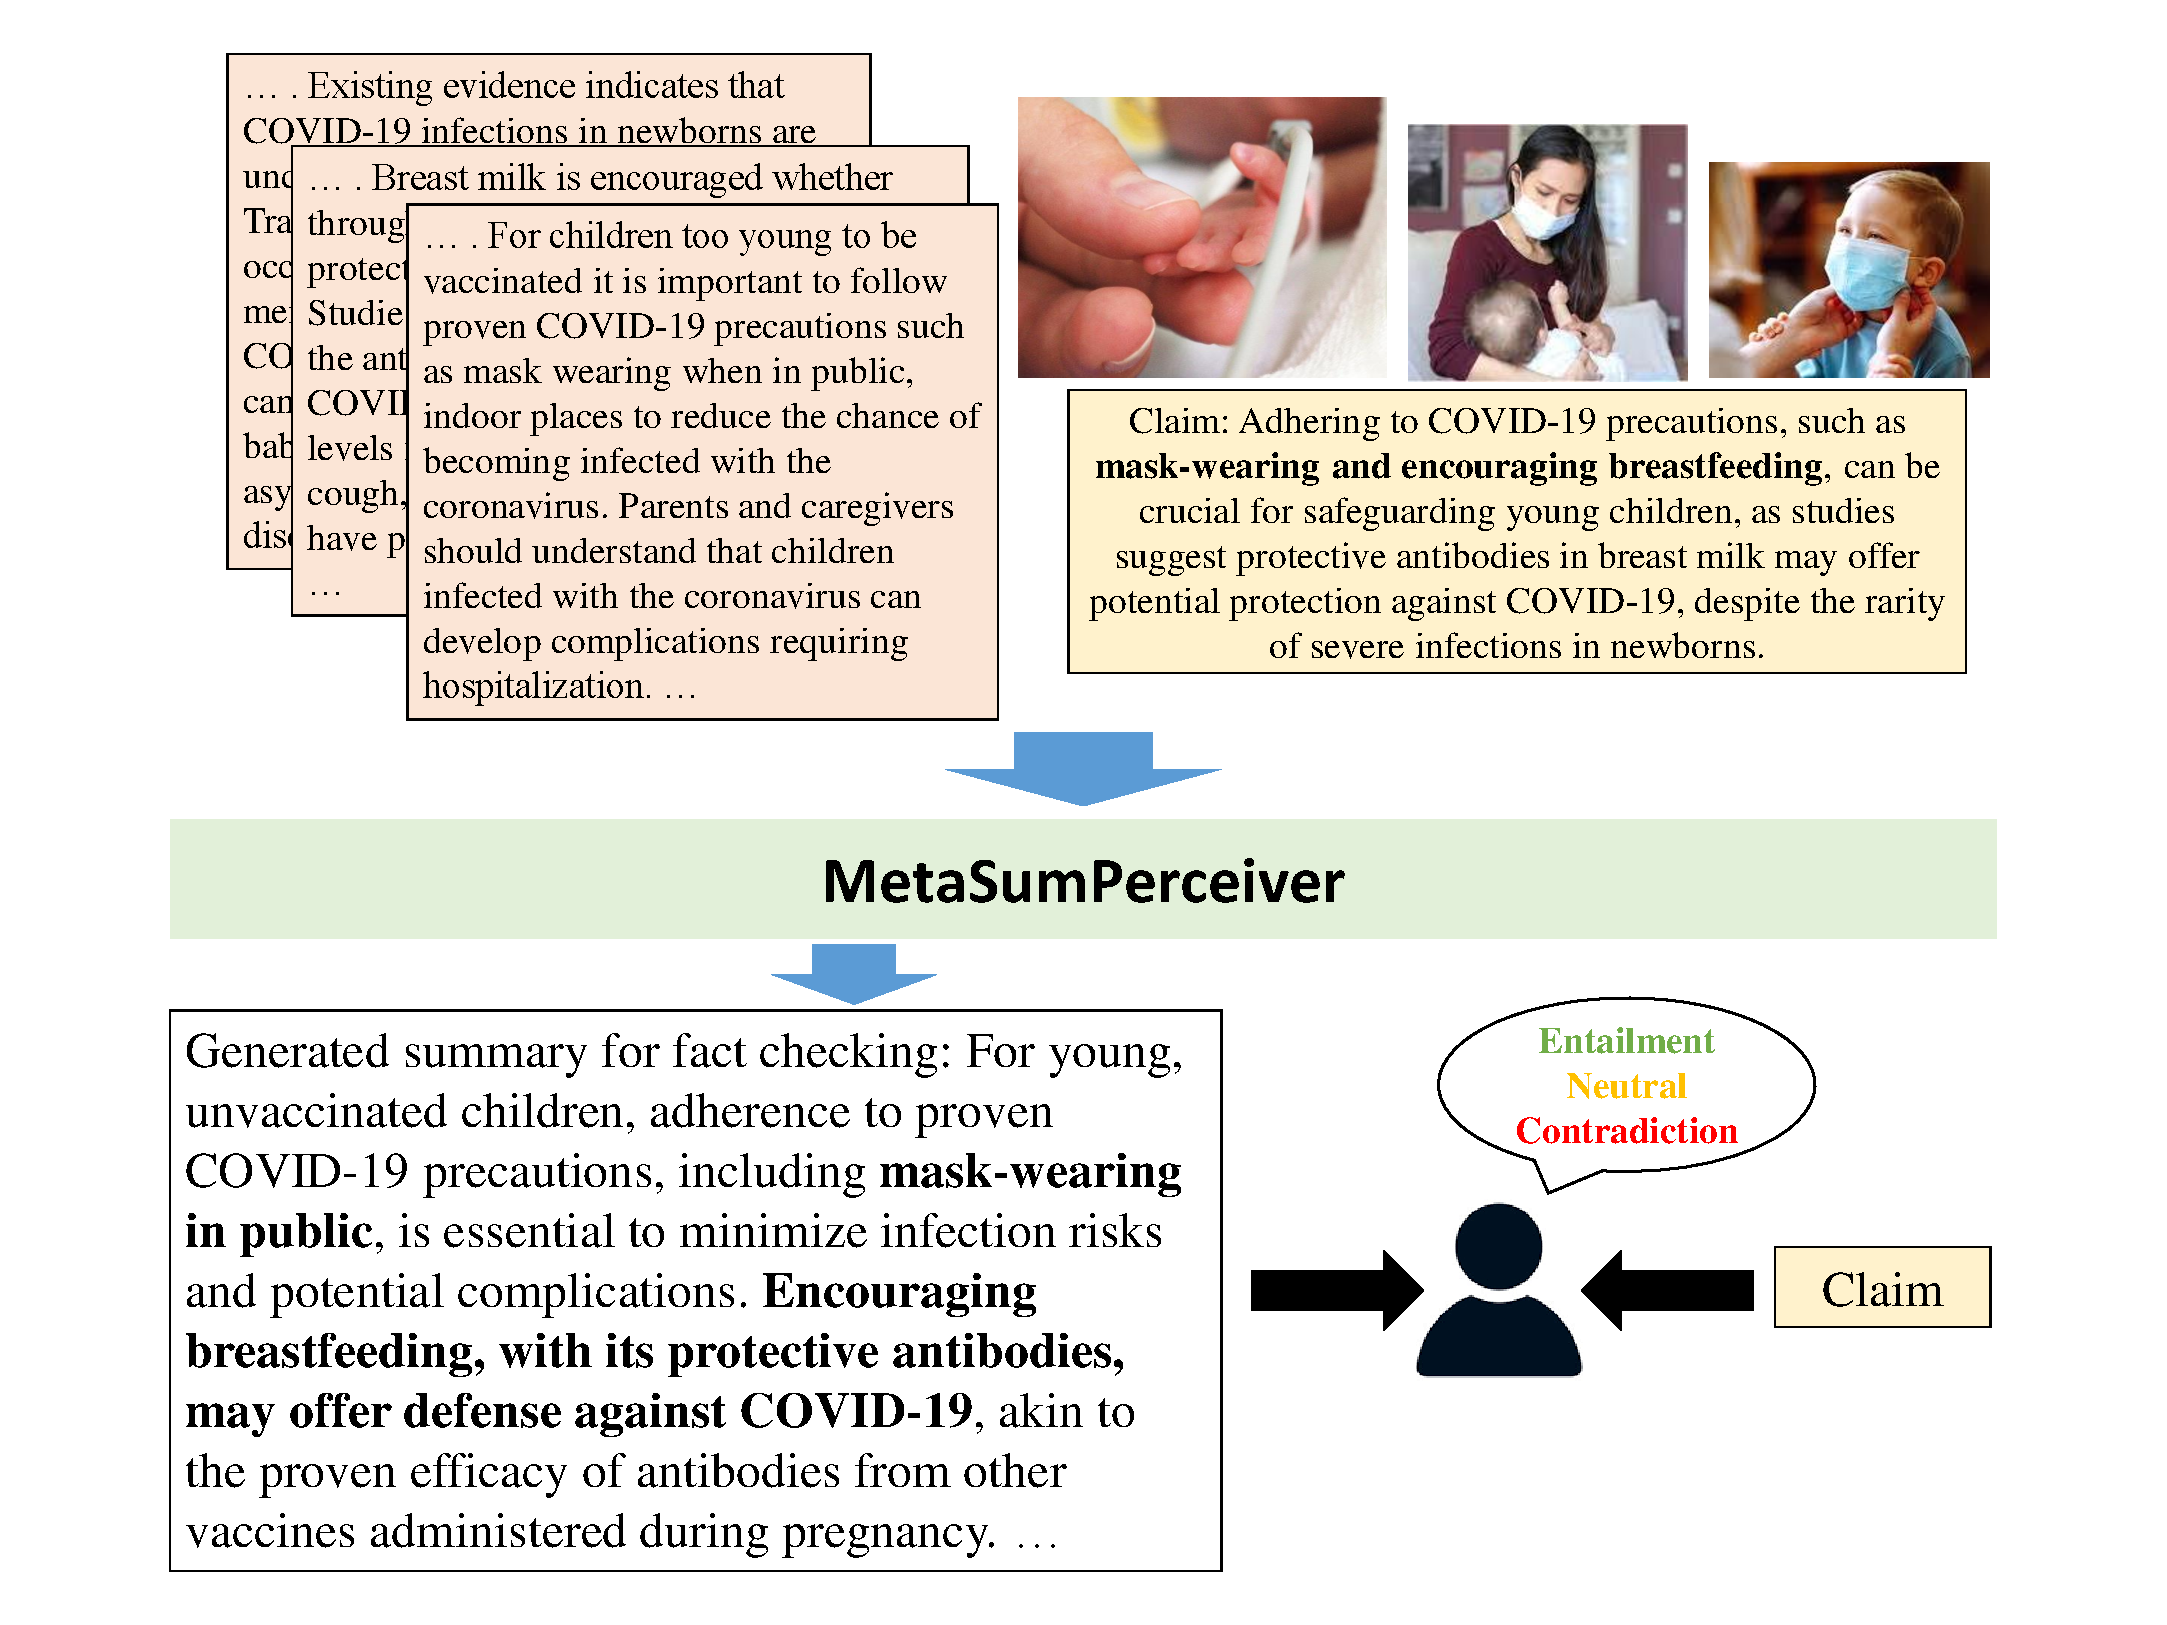
\includegraphics[width=\textwidth,height=0.5\textwidth,keepaspectratio]{images/metasumperceiver.pdf}
  \caption{Overview of MetaSumPerceiver: Using inputs such as documents, images, and claims, MetaSumPerceiver generates summaries to facilitate fact-checking. In this example, the summary for fact-checking provides evidence and establishes that the claim in question is entailed by the evidence.}
  \label{fig:metasumperceiver_overview}
\end{figure*}

To overcome the challenge of fact-checking with multimodal multi-document sources, we propose the~\textbf{MetaSumPerceiver} model in Figure~\ref{fig:metasumperceiver_overview}, where the input consists of a claim, a set of documents and images, and the objective is to generate a summary that expedites the fact-checking process for humans. we initially train the perceiver model~\cite{jaegle2022perceiver,jaegle2022perceiver_1} with a summarization model~\cite{lewis2019bart}. Subsequently, to produce the summary for fact-checking, we employ a proxy reward mechanism to update the summarizer to ensure the generation of an accurate and relevant summary with necessary evidence. Then, to train~\textbf{MetaSumPerceiver} to generate summaries useful for human fact-checking, we assess the utility of our summaries at performing entailment~\cite{inproceedings, poliak2020survey, bowman-etal-2015-large}, a closely aligned task to fact-checking. our work is orthogonal to prior work in entailment, in that rather than learning to predict the entailment label for the premise-hypothesis pair, we seek to generate the premise for a specific claim from a pool of multimodal data. In order to support research on the task of multimodal multi-document fact-checking, we also introduce the~\textbf{KG2Claim} approach outlined in Figure~\ref{fig:amrkg2claim}. This approach takes a multimodal multi-document knowledge graph as input and aims to create claims that incorporate this diverse information through multimodal coreference resolution~\cite{otmazgin2022fcoref, cattan2021realistic, caciularu-etal-2021-cdlm-cross}. 

\begin{figure*}
\centering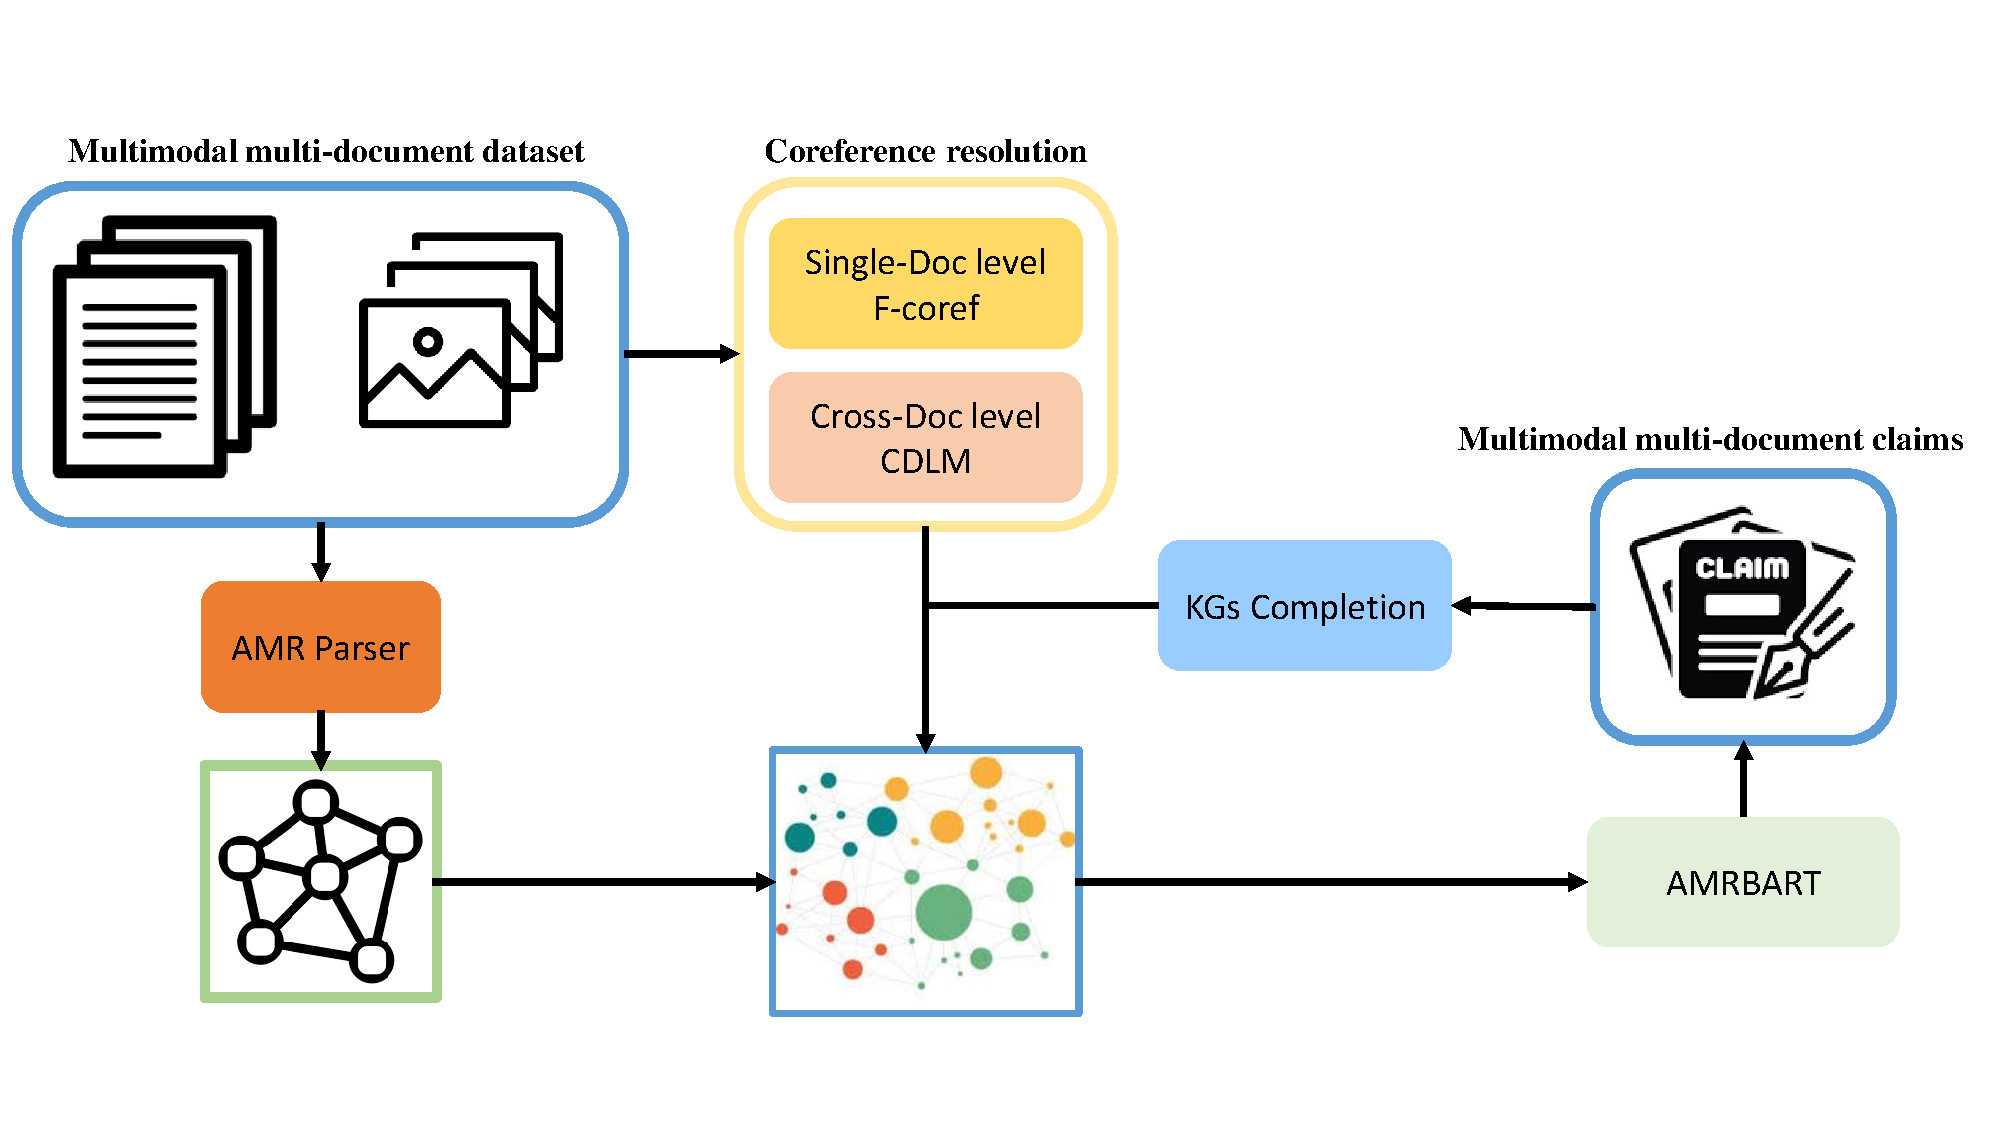
\includegraphics[width=\textwidth,height=0.5\textwidth,keepaspectratio]{images/amrkg2claim.pdf}
  \caption{Pipeline of KG2Claim: The elements encompass an AMR parser, single-document and cross-document coreference resolution, Knowledge graphs completion with LLMs, and AMRBART, generating the multimodal multi-document claims.}
  \label{fig:amrkg2claim}
\end{figure*}

To assess the efficiency of the~\textbf{MetaSumPerceiver}, we employ our~\textbf{KG2Claim} method for the fact-checking task, evaluate it against the MOCHEG benchmark~\cite{Yao_2023}, and introduce a new benchmark called Multi-News-Fact-Checking. Multi-News-Fact-Checking benchmark involves claims and entailment labels supported by evidence from multiple documents. Our results indicate significant enhancements compared to existing baselines.

The major contributions of this thesis are as follows:
\begin{itemize}
  
    \item We present an innovative approach for multimodal multi-document summarization specifically designed for fact-checking applications.

    \item We introduce a claim generation method tailored for disinformation detection tasks, with a focus on handling multimodal multi-document information.

    \item We release the Multi-News-Fact-Checking dataset, to support the multi-document fact-checking summarization task.
  
    \item We perform detailed experiments and ablations of our approach and loss functions which clearly demonstrate the superiority of our approach over existing methods.
  
\end{itemize}

    \chapter{Review of Literature} \label{ch:lit_review}
        \section{Knowledge Representation} \label{se:AMR}
            Abstract Meaning Representation (AMR)~\cite{garg2018stochastic, ballesteros2017amr, lyu2018amr} functions as a robust semantic representation language, employing rooted, labeled, directed, and acyclic graphs to encapsulate entire sentences. This representation brings forth two pivotal advantages. Firstly, AMR serves as a conduit for semantic representation, adept at capturing the intricate structural nuances within sentences, thereby delineating the relationships that underpin various entities. Secondly, AMR seamlessly integrates semantic role labeling, shedding light on the nuanced roles assumed by different words in a sentence, such as agents, patients, or locations.

The strength of AMR lies in its holistic approach to language representation. AMR not only enhances semantic clarity but also facilitates a more profound understanding of the relationships inherent in linguistic expressions. This depth is particularly valuable when unraveling complex narratives or dissecting intricate layers of meaning within the text. Comparatively, when juxtaposed with Information Extraction (IE)~\cite{zheng2023survey, 10221008}, AMR emerges as a comprehensive information tool. Unlike IE, which is confined to extracting predefined information from textual sources and struggles with untrained sentences, AMR exhibits the versatility to analyze diverse sentences through its nuanced semantic representation.

Harnessing the advantages of AMR, this thesis employs IBM AMR parser~\footnote{\url{https://github.com/IBM/transition-amr-parser}} for extracting textual sources. By doing so, it not only dissects the relationships between events and entities but also benefits from the inherent depth that AMR brings to the semantic analysis of linguistic expressions. 

        \section{Coreference Resolution} \label{se:coref}
            Coreference resolution is the task of finding all expressions that refer to the same event and entity in a text. It is an important step for a lot of higher-level NLP tasks that involve natural language understanding such as document summarization, question answering, and information extraction. Recent research has introduced innovative approaches to sentence-level coreference resolution~\cite{grenander2023sentenceincremental,10.1162/tacl_a_00543} and document-level coreference resolution~\cite{10.1145/3539597.3573038,10.1007/978-3-031-40286-9_34}. The primary technology entails detecting candidate mentions, encoding them into vector representations, and identifying coreference relations by employing a Multilayer Perceptron (MLP) classifier to process the representations of each mention and past entities~\cite{Liu2023il}. Notably,~\citet{joshi2020spanbert} established the SpanBERT model, achieving state-of-the-art performance in coreference resolution. Furthermore,~\citet{yao-etal-2023-learning} developed a model inspired by SpanBERT, designed to learn and integrate multiple representations from both event alone and event pair. 

We implement coreference resolution at both the single-document and cross-document levels. For single-document coreference resolution, we employ F-coref~\cite{otmazgin2022fcoref} to identify the same entities on a sentence-by-sentence basis. Subsequently, for the cross-document coreference resolution, we utilize CDLM~\cite{caciularu-etal-2021-cdlm-cross} to extract coreferent entities. This crucial step serves to establish connections between identical entities within the knowledge graphs. Moreover, it enables tracking the specific document in which these entities are mentioned.


        \section{Knowledge Graph Completion} \label{se:KGC}
            In knowledge graphs (KGs), latent relationships between events and entities often result in unknown connections, necessitating approaches to comprehend the missing information; this gap is addressed through knowledge graph completion~\cite{SHEN2022109597,Lin_Liu_Sun_Liu_Zhu_2015,Shi_Weninger_2018}, a method that predicts and fills in missing relationships or edges between entities, thereby enhancing the overall comprehensiveness of the knowledge graph.

~\citet{NIPS2013_1cecc7a7} invented TransE to construct entity and relation embeddings by treating relations as translations from head entity to tail entity. Inspired by~\citet{mikolov2013distributed}, TransE learns vector embeddings for entities and relationships, placing them in $\mathbb{R}^k$. The fundamental concept behind TransE is that the relationship between two entities is akin to a translation between their embeddings, expressed as $h+r\approx t$ when $(h,r,t)$ holds, where $h$ represents the head entity, $t$ represents the tail entity and $r$ represents the relationship from the head entity to tail entity, respectively. However, due to challenges in modeling 1-to-N, N-to-1, and N-to-N relations,~\citet{10.5555/2893873.2894046} introduced TransH to allow entities to have distinct representations in different relations. Incorporating BERT~\cite{devlin2019bert} into the knowledge graph completion task,~\citet{yao2019kgbert} developed KG-BERT. This model takes the entity and relation descriptions of a triple as input, computes the scoring function for the triple using the KG-BERT language model, and predicts unknown relationships.~\citet{zhang2023making}  incorporate the helpful KGs structural information into the LLMs, aiming to achieve structural-aware reasoning in the LLMs. They first transfer the existing LLMs paradigms to structural-aware settings and propose a knowledge prefix adapter to predict the unknown relationships.

To address this challenge in KGs, we utilize Vicuna~\cite{vicuna2023} to identify hidden relationships within each claim. Furthermore, we incorporate additional claims to elucidate latent connections in the KGs, enhancing the information within knowledge graphs. This process aids in a more comprehensive understanding of events and entities during the generation of multimodal multi-document claims.

        \section{Perceiver} \label{se:perceiver}
            The perceiver architecture~\cite{jaegle2021perceiver} in Figure~\ref{fig:perceiver} enables scaling transformers to input sequences of arbitrary lengths, by reducing the memory footprint in standard self-attention. Perceiver is an architecture grounded in attentional principles, designed to handle high-dimensional inputs and multimodal combinations without relying on domain-specific assumptions. It employs a cross-attention module to map a high-dimensional input byte array to a fixed-dimensional latent bottleneck. Subsequently, it processes this bottleneck through a deep stack of Transformer-style self-attention blocks in the latent space. The perceiver engages in an iterative process of attending to the input byte array by alternating between cross-attention and latent self-attention blocks.

Follow-up works, such as Perceiver IO~\cite{jaegle2022perceiver}, adapt the original model by presenting a versatile architecture adept at processing data from various settings while ensuring linear scalability with input and output dimensions. The model has demonstrated strong performance on many downstream tasks, including the GLUE language benchmark~\cite{wang2019glue}, Sintel optical flow estimation~\cite{Butler:ECCV:2012}, and others all without the need for explicit multiscale correspondence mechanisms. 

Uni-Perceiver v2~\cite{Li_2023_CVPR} stands out as the first generalist model capable of efficiently handling major large-scale vision and vision-language tasks. Notably,~\citet{Li_2023_CVPR} can directly manage downstream tasks without requiring task-specific adaptation, such as image classification, object detection, image-text retrieval, and image captioning. Our method relies on~\citet{Li_2023_CVPR} to process a variable number of arbitrarily long text documents and images. We use the model in sequence with a summarization model to generate a multimodal summary.

\begin{figure*}
\centering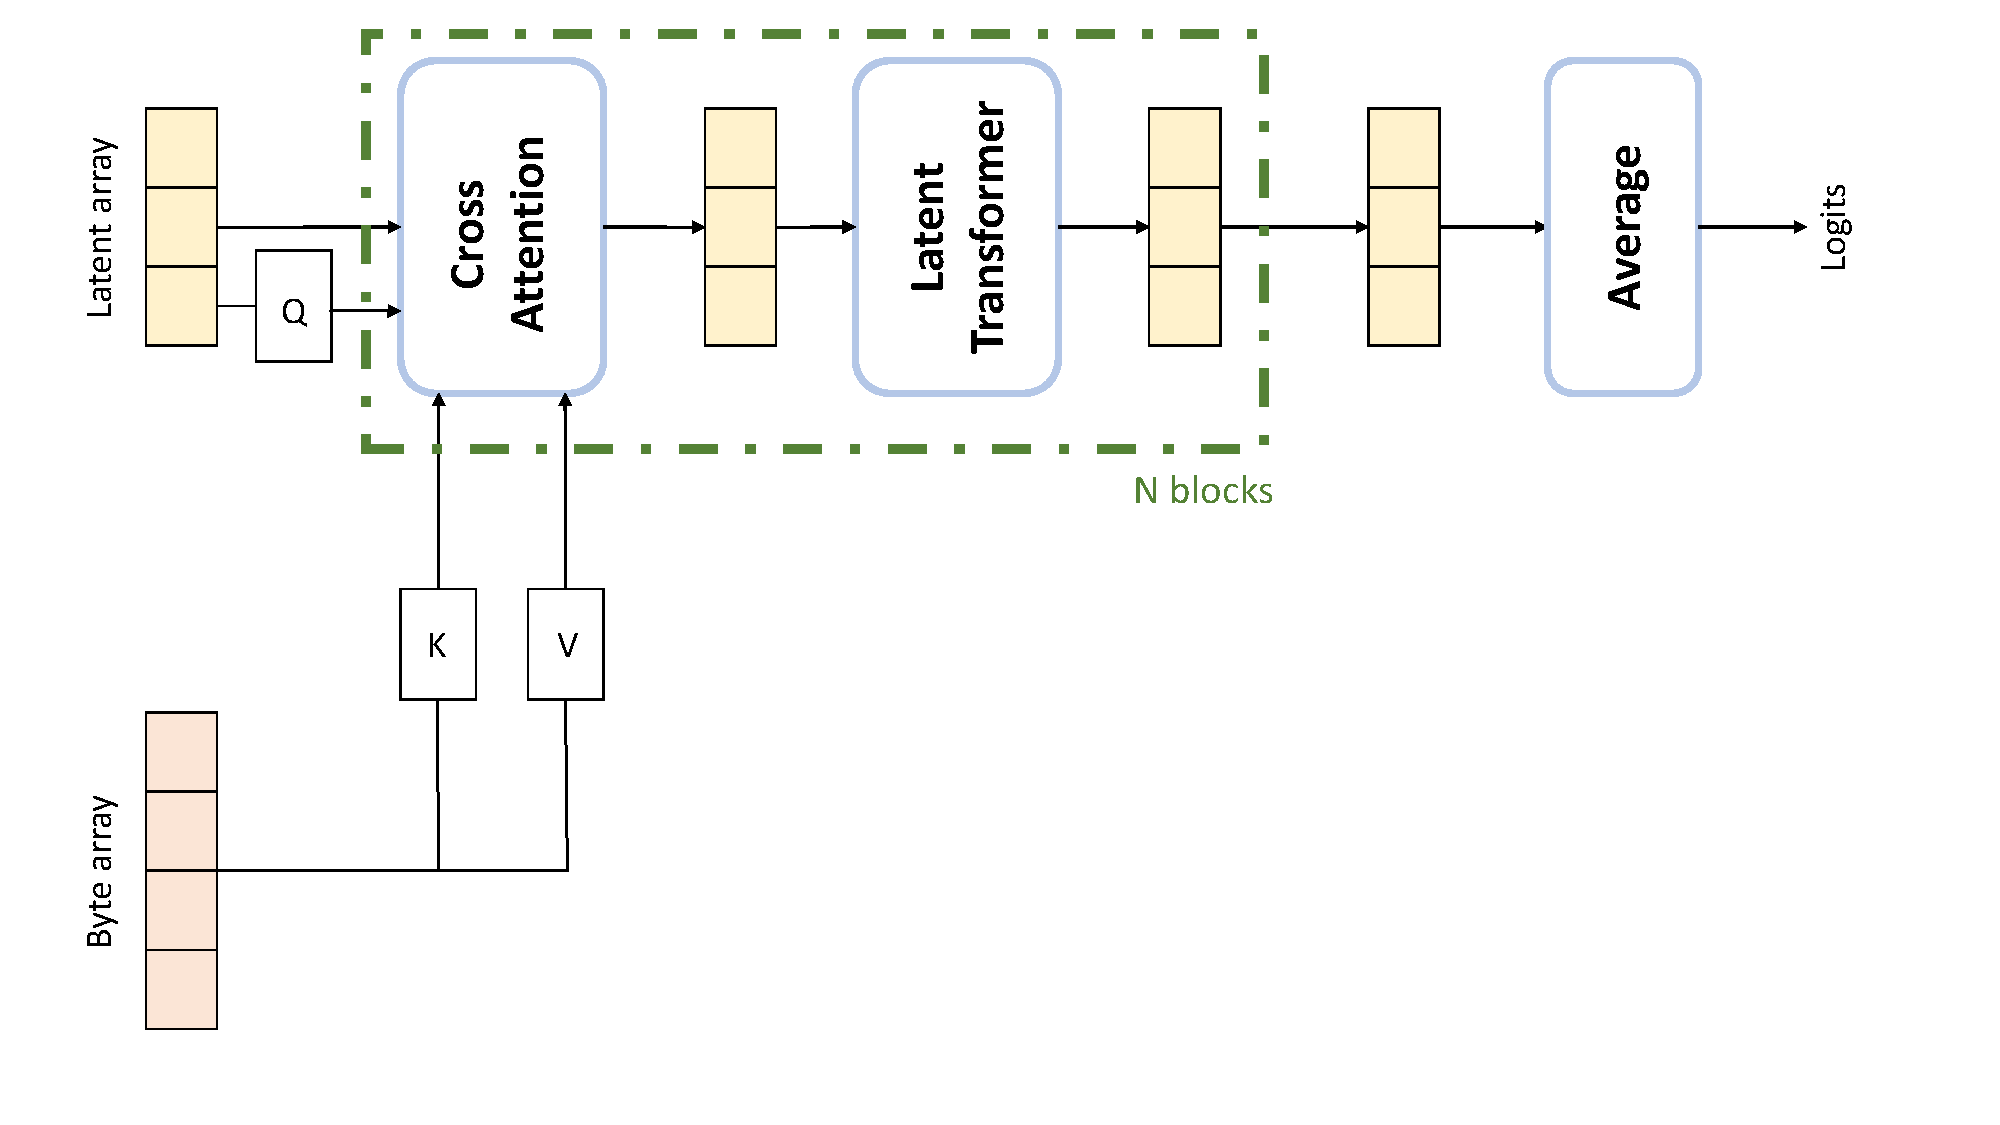
\includegraphics[width=\textwidth,height=\textwidth,keepaspectratio]{images/perceiver.pdf}
  \caption{The perceiver architecture.}
  \label{fig:perceiver}
\end{figure*}

        
        \section{Multimodal Summarization} \label{se:multi-sum}
            Recently, a number of approaches have been proposed for generating summaries of multimodal content.~\citet{111_inproceedings} use input audio to generate textual summaries.~\citet{7926698} extract textual summaries from annotated and summarized videos.~\citet{article,zhu-etal-2018-msmo} propose an integrated approach which utilizes both textual and visual modalities as inputs and produce multimodal outputs summarizing text and video.~\citet{palaskar-etal-2019-multimodal} propose to generate abstractive summaries from open-domain videos. Despite this recent progress, existing models continue to struggle with capturing complementary information from multiple modalities. Unlike prior work in this space, we seek to generate textual summaries of evidence from multiple modalities for purposes of fact-checking.

        \section{Learning from Feedback} \label{se:lear-feed}
            Recent advancements in LLMs have revolutionized the AI landscape~\cite{touvron2023llama1, touvron2023llama, driess2023palme, openai2023gpt4}. However, because they are mostly trained on data scraped from the web LLMs sometimes produce undesired outcomes, including generating biased or harmful content~\cite{10.1145/3442188.3445922}. Recognizing the importance of aligning LLMs with human values,   has led to efforts in supervised fine-tuning (SFT) with ethical guidelines~\cite{alpaca}. While these efforts demonstrate the potential of integrating human feedback into training using reinforcement learning for user-tailored tasks~\cite{ouyang2022training, bai2022training}, training LLMs to reflect human values is quite challenging. 

In our work, we adopt the idea of training language models with feedback. However, rather than relying on a human fact-checker, we utilize a surrogate reward model (an entailment model) to stand in the place of a human fact checker, in order to fine-tune the summarizer to generate summaries that give evidence for fact-checking specific claims through Proximal Policy Optimization (PPO)~\cite{schulman2017proximal, zheng2023secrets}.
        \section{Training Strategy: from BERT to DeBERTa V3} \label{se:training-strategic}
            ~\citet{devlin2019bert} employs two key unsupervised training tasks: Masked Language Model (MLM) and Next Sentence Prediction (NSP), which collectively contribute to the model's ability to understand contextualized word representations and relationships between sentences. The MLM task involves randomly masking some words in a sentence and training the model to predict the masked words based on the context of the surrounding words. This helps BERT learn bidirectional contextual representations, capturing the meaning of words in the context of the entire sentence. The NSP task, on the other hand, involves predicting whether one sentence follows another in a document. This task encourages the model to understand the relationships and coherence between sentences, enabling BERT to grasp the broader context of a document. By combining these tasks during pre-training, BERT learns rich contextualized representations that make it highly effective for a wide range of natural language processing tasks.

To enhance performance,~\citet{clark2020electra} suggests replacing the pretraining task with the "Replaced Token Detection" (RTD) task, akin to generative adversarial networks (GANs). In the RTD task, the objective is to discern whether a given token is original or not. Results indicate that weight sharing outperforms the MLM task because the RTD task updates only the input token embedding in the discriminator. DeBERTa V3 in Figure~\ref{fig:deberta} integrates the DeBERTa model with the RTD task, enhancing relative position embedding and emphasizing absolute position embedding in the final layer. Comparative results demonstrate DeBERTa's superiority over BERT. Moreover, DeBERTa V3 retains the DeBERTa model with the RTD task, achieving the best performance in GLUE with an impressive 91.37\% average score according to experiments. In our work, we primarily employ DeBERTa V3 as our entailment model to help determine whether a claim is entailed by a summary or not.
        \section{Prompting from LLMs} \label{se:prompt}
            The direct impact of a prompt or prompt strategy on model outputs, as well as the modification of LLMs' billions of parameters during re-training, are both active areas of research~\cite{liu2021pretrain,sanh2022multitask}. Recent research~\cite{xing2023prompt,white2023prompt,lian2023llmgrounded} provides some insights into effective prompt design strategies.~\citet{brown2020language} demonstrated that examples significantly enhanced GPT-3's performance across tasks such as question answering and language translation. We focus on designing effective prompts for fact-checking. Additionally, we release our prompted results as a pseudo-labeled dataset to establish a benchmark on this task.

\begin{figure*}
  \centering
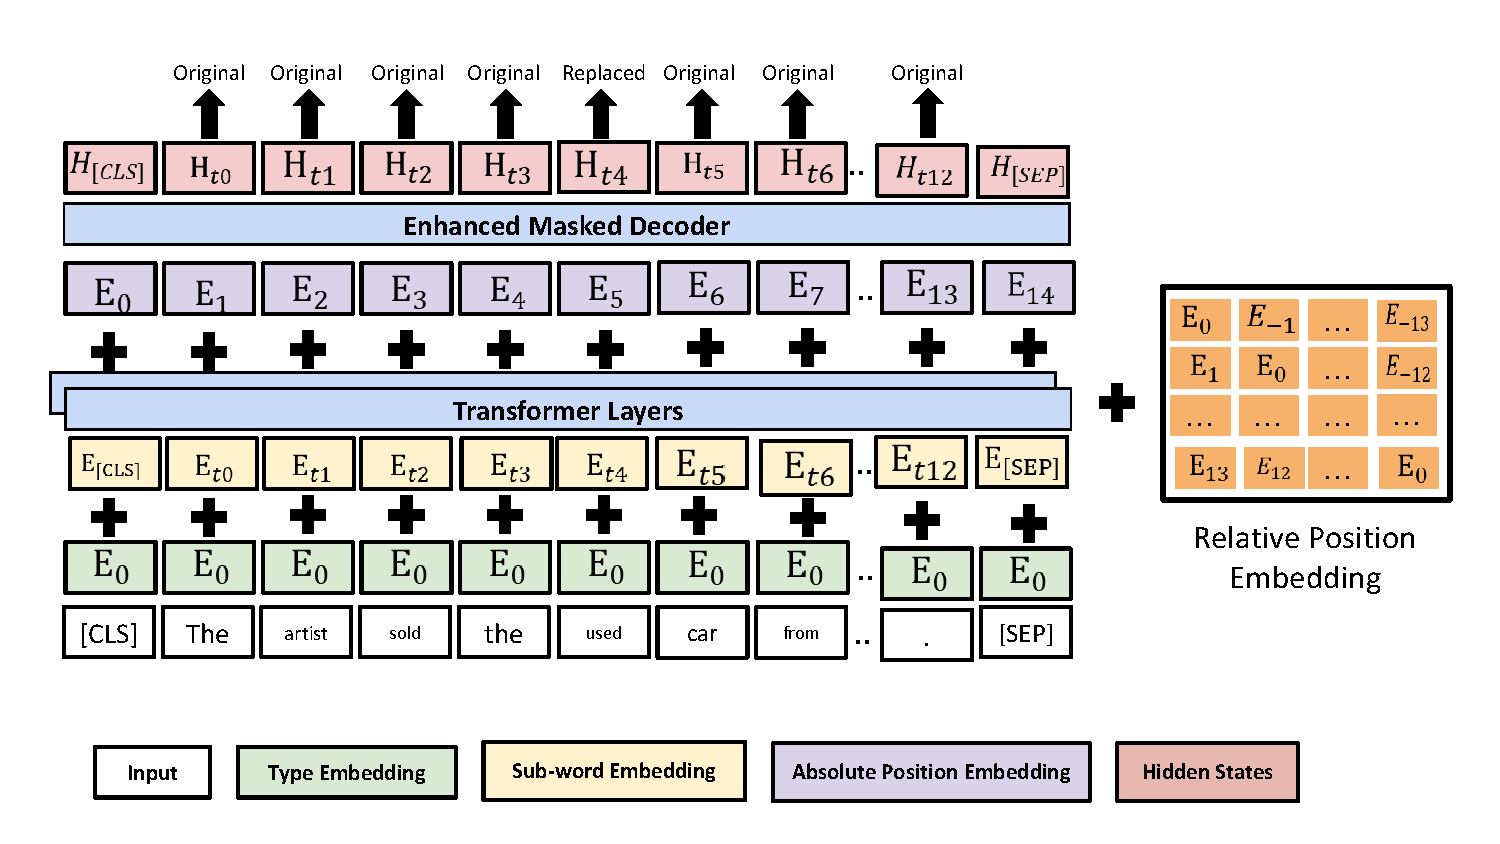
\includegraphics[width=\textwidth,height=\textwidth,keepaspectratio]{images/deberta.pdf}
  \caption{Overview of training strategy in DeBERTa V3: This figure involves passing sub-word embedding which is token embedding through several transformer layers, adding it to position embedding. It then goes through another transformer layer, followed by training using replacing token detection. The position embedding is divided into absolute and relative components. Absolute follows the original BERT, emphasizing absolute word positions. Relative, on the other hand, emphasizes relative positions. This approach highlights absolute word positions in the final layer.}
  \label{fig:deberta}
\end{figure*}
            
    \chapter{Methodologies} \label{ch:methods}
                
        \section{Evidence Summarization Model (MetaSumPerceiver)} \label{se:ESM}

            \subsection{Model Training Strategy} \label{subse:MTS}
                We explain the details of our approach,~\textbf{MetaSumPerceiver} in Figure~\ref{fig:metaover}, as well as how we construct our Multi-News-Fact-Checking dataset as illustrated. We also describe the preprocessing steps for both text and image data, the components of our model, and the reinforcement learning methodology we applied to train~\textbf{MetaSumPerceiver}. Our approach is capable of summarizing multiple multimodal documents consisting of arbitrarily long texts and images. Specifically, we use $x_C$, $x_D$, and $x_I$ to represent embeddings for claims, documents, and images, respectively.

\begin{figure*}
  \centering
  \includegraphics[width=\textwidth, height=\textwidth, keepaspectratio]{images/pipeline_3.2.pdf}
  \caption{Overview of MetaSumPerceiver: This figure illustrates the process of generating a summary for fact-checking using MetaSumPerceiver, integrating a fixed entailment model for accurate truthfulness labeling. Furthermore, it highlights how PPO is employed to continually refine the summary during the fact-checking process.}
  \label{fig:metaover}
\end{figure*}

For the textual data, we use BART~\cite{lewis2019bart}~\footnote{ \url{https://huggingface.co/facebook/bart-large-cnn}.}  to obtain text embeddings following~\cite{devlin-etal-2019-bert,liu2019roberta}. As a result, each input text is transformed into a set of token embeddings $x_C \in \mathbb{R}^{n \times D}$ and $x_D \in \mathbb{R}^{m \times D}$, where $n$ and $m$ are the number of tokens and $D$ is the dimension of embedding. We use CLIP (ViT-G-14)~\cite{radford2021learning} to extract visual features for the images. Finally, each input image undergoes a transformation, resulting in a set of visual embeddings. $x_I \in \mathbb{R}^{k \times D}$, where $k$ is the number of tokens and $D$ is the dimension of the embedding.

Our goal is to generate a textual summary of a set of multimodal documents that enables a fact-checker to determine the veracity of a claim. In order to select relevant visual content from the images, we begin by performing a cross-attention between the images and the claim:

\begin{equation}
  \begin{array}{l}
    X_{IC}= ATTN(Q_{x_C}, K_{x_I}, V_{x_I}) \;,
  \end{array}
\end{equation}

where the query $Q_{x_C}$ is the claim's sequence of embeddings and $K_{x_I}$ and $V_{x_I}$ are the embedding sequences of visual tokens from the images. We project $X_{IC}$ into the document embedding $X_D$, which serves as the input for~\textbf{MetaSumPerceiver}.

The output from the cross-attention block, $X_{IC}$, is initially projected by a linear projection layer with the weight $\theta$. It is then concatenated with $x_D$, as depicted in the subsequent equation:

\begin{equation}
  \begin{array}{l}
  X_{ICD} = 
  \begin{bmatrix}
    proj(X_{IC}, \theta)^\intercal , X_D ^\intercal 
  \end{bmatrix}^\intercal,
  \end{array}
\end{equation}

where $X_{ICD}$ will be the input to~\textbf{MetaSumPerceiver}. Prior to training our full model, we pretrain our attention block and summarization model using the Multi-News dataset's human written summaries using the cross-entropy loss function:

\begin{equation}
  \begin{array}{l}
    \mathcal{L}_{\text{sum}} = -\sum_{t=1}^{T} \sum_{i=1}^{N} y_{t_i} \log(\hat{y}_{t_i}),
  \end{array}
\end{equation}

where $T$ represents the sequence length, $N$ is the vocabulary size, and $y_{t_i}$ and $\hat{y}_{t_i}$ denote the ground truth and predicted probabilities of token $i$ at time step $t$, respectively. In the remaining text, we omit the summation over the vocabulary for conciseness.
            \subsection{Reward Model for Fine-tuning the Summarizer} \label{subse:reward}
                To enhance the summarizer's ability to produce summaries that provide the evidence needed for fact-checking claims, we adopt the concept of training a language model using feedback with reinforcement learning. After pretraining the perceiver and summarization models, we employ reinforcement learning with an entailment model serving as a surrogate for a human fact-checker as feedback. We first exclusively apply reinforcement learning (RL) to the perceiver. Subsequently, we unfreeze the summarizer and continue training end-to-end with both the perceiver and summarizer. We illustrate our fine-tuning process in Figure~\ref{fig:rl_ppo}. Contrary to the approach in reinforcement learning from human feedback, which necessitates a human arbitrator to score the model's outputs, in this study, we train a reward model to act like a human fact-checker to guide the summarizer in producing summaries for fact-checking instead.

\begin{figure*}
  \centering
  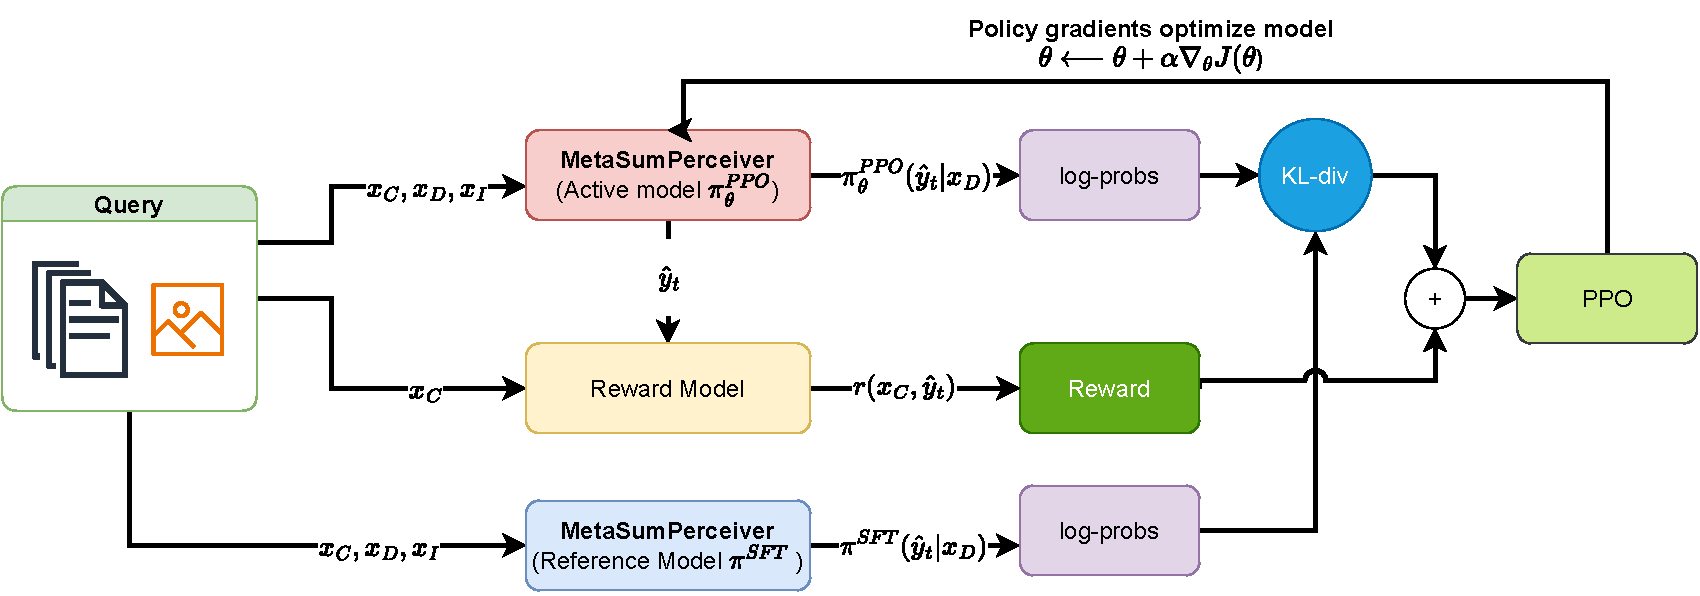
\includegraphics[width=\textwidth,height=\textwidth,keepaspectratio]{images/ppo.pdf}
  \caption{The Proximal Policy Optimization (PPO) workflow begins with the summarizer creating a response based on the input query. The reward model then evaluates this query-response pair that outputs a scalar reward. Meanwhile, the process calculates the KL-divergence based on the likelihood of token sequences in the response using both an active model being fine-tuned currently and a pre-trained reference model. The KL-divergence serves as a reward measure, ensuring responses from the active model are aligned with the reference model. Conclusively, PPO updates the active model's parameters, relying on the result of the reward model's output and the KL-divergence's value.}
  \label{fig:rl_ppo}
\end{figure*}

We utilized a comprehensive dataset consisted with MultiNLI~\cite{N18-1101}, Fever-NLI~\cite{Thorne18Fever}, and Adversarial-NLI (ANLI)~\cite{nie-etal-2020-adversarial}, encompassing a total of 763,193 premise-claim pairs. Leveraging this dataset, we fine-tuned DeBERTa V3~\cite{he2023debertav3} for the task of entailment classification using cross-entropy loss. Serving as an entailment classifier, this model achieves accuracy rates of 90.3\%, 77.7\%, and 57.9\% in the MultiNLI, Fever-NLI, and ANLI evaluation datasets, respectively. We define the score from the reward model as the probability of the ground-truth label given both the claim (as the hypothesis) and the generated summary for fact-checking (as the premise). The formulation for the score from the reward model can be formulated as:

\begin{equation}
  \begin{array}{l}
    r(x_C, \hat{y}_t) = P(y_{gt}|{x_C, \hat{y}_t}) - 
    0.5 * \Sigma_{y_{gt} \neq y_{pred}} P(y_{pred}|{x_C, \hat{y}_t}),
  \end{array}
\end{equation}

where $x_C$, $\hat{y}_t$, $y_{gt}$ and $y_{pred}$ denote the claim, the generated summary, the groud-truth label of the claim, and the predicted label of the claim, respectively. The value of $P(y_{\{gt,pred\}}|x_C,\hat{y}_t)$ is derived from the trained entailment classifier. The primary objective behind this reward function is to maximize the likelihood that the generated summary for fact-checking contains the facts necessary for the model to predict the claim's ground truth label.

We employ PPO as our policy gradient method for reinforcement learning. PPO adds an additional term to the reward function, which imposes a penalty determined by the Kullback-Leibler (KL) divergence between the trained RL policy summarizer, $\pi^{PPO}_{\phi}$, and the initial supervised summarizer $\pi^{SFT}$. This cumulative reward is described as follows:

\begin{equation}
  \begin{array}{l}
    r_{total} = r(x_C, \hat{y}_t) - 
    \eta KL(\pi^{PPO}_{\phi}(\hat{y}_t|x_D), \pi^{SFT}(\hat{y}_t|x_D)),
  \end{array}
\end{equation}

where $\eta$ represents the KL reward coefficient, which determines the magnitude of the KL penalty, we set it to 0.2 for our model. This coefficient functions as an entropy boost, enhancing exploration throughout the policy domain and urging the model to engage in a diverse set of actions rather than the one currently considered the best. In addition, it inhibits the policy from rapidly committing to a singular strategy, and this encourages outputs from the RL fine-tuned model to not deviate too far from the original model. ~\textbf{MetaSumPerceiver} is optimized through PPO based on the policy gradient methods that optimize the policy of the model using gradient ascent. The update rule for the policy gradient is given as: 

\begin{equation}
  \begin{array}{l}
    \theta \longleftarrow \theta + \alpha \nabla_{\theta} J(\theta),
  \end{array}
\end{equation}

where $\alpha$ and $J_{\theta}$ denote the learning rate and the expected return under policy $\pi_{\theta}$ from the model, respectively.



            \subsection{Multi-News-Fact-Checking Dataset} \label{subse:MNFCD}
                In order to train our system, we need a dataset of claims whose facts are drawn from multiple documents along with the entailment label of each claim. We build our dataset on top of the Multi-News summarization dataset \cite{alex2019multinews}, which contains sets of multiple text documents along with human-written summaries of each set. Because the Multi-News dataset doesn't have claims specifically made for fact-checking and lacks images for the news articles, we use Llama-2-70b~\cite{touvron2023llama}. We ask it to create labeled claims from each set of documents and get news images from Google. In each group of Multi-News documents, we use the human-written multi-document summary to generate 30 claims (ten of each type), giving us a dataset of 1,291,168 labeled claims. Additionally, we collect 111,905 images for our multimodal multi-document dataset. The prompts include sections with a task description, example, and instructions, which are fully detailed in appendices~\ref{ase:app_prompt_llama2}.


%Because the Multi-News dataset lacks claims specifically tailored for fact-checking tasks and the images for the news articles, we prompt Llama-2-70b~\cite{touvron2023llama} to generate labeled claims from each set of documents and scrape the news images from Google. Within each group of Multi-News documents, we leverage the human-written multi-document summary to generate 30 claims (ten of each entailment type), resulting in a dataset of 1,291,168 labeled claims. In addition, we scrape the 111,905 images for our multimodal multi-document dataset. The specific prompts contain sections containing a task description, example, and instructions. We show the complete prompts in the appendices~\ref{ase:app_prompt_llama2}.


        \section{Multimodal Multi-document Claims Generation Method (KG2Claim)} \label{se:MMCGM}
        
            \subsection{Multimodal Coreference Resolution} \label{subse:EECR}
                We have a two-step approach for the coreference resolution task. The initial step involves single-document coreference resolution, where we utilize F-coref~\cite{otmazgin2022fcoref}. Subsequently, the second step focuses on cross-document coreference resolution, where we employ CDLM~\cite{caciularu-etal-2021-cdlm-cross}. In the context of single-document coreference resolution, F-coref emerges as a Python package designed for swift, precise, and user-friendly English coreference resolution. Drawing inspiration from s2e~\cite{kirstain-etal-2021-coreference}, F-coref introduces parallelism through batching, thereby reducing unnecessary computations like padded tokens. Similar to other neural coreference models, F-coref evaluates each pair of spans in the text for potential co-reference.

The architecture of F-coref encompasses three key components: (1) Longformer~\cite{beltagy2020longformer}, serving as a contextualized encoder; (2) a parameterized mention scoring function denoted as $f_m$; and (3) a parameterized pairwise antecedent scoring function labeled as $f_a$. To determine the coreference likelihood between any pair of spans, the model initiates by encoding the text through Longformer, resulting in vectors $x_1,...,x_n$. Subsequently, for each potential span $q$ = $(x_k, x_l)$, the mention scoring function $f_m(q)$ evaluates the probability of $q$ (the "query") being a mention. For a given pair of spans $c = (x_i, x_j)$ and $q = (x_k, x_l)$, where $c$ ("candidate") precedes $q$, the pairwise antecedent scoring function $f_a(c, q)$ assesses the likelihood of $c$ being an antecedent of $q$. In practical terms, to mitigate the complexity of $O(n^4)$, the antecedent function scores only the top $\lambda T$ spans with the highest mention scores (where $T$ represents the number of tokens). Ultimately, the final pairwise score for a coreference link between $c$ and $q$ comprises the scores indicating the likelihood of $q$ and $c$ being mentioned, along with the probability of $c$ being an antecedent of $q$:

\begin{equation}
  F(c,q) =
    \begin{cases}
      f_m(c)+f_m(q)+f_a(c,q) & \text{$c \neq \varepsilon$}\\
      0 & \text{$c = \varepsilon$},
    \end{cases}       
\end{equation}

where $\varepsilon$ is the null antecedent. The computation of $f_m$ and $f_q$ for the entire sequence can be efficiently batched.

In the cross-document coreference resolution task, we employ CDLM~\cite{caciularu-etal-2021-cdlm-cross} in Figure~\ref{fig:cdlm}, a pretraining approach designed for multi-document language modeling. This method incorporates two key concepts: (1) pretraining over sets of related documents with overlapping information and (2) pretraining utilizing a dynamic global attention pattern over masked tokens to reference the entire cross-text context. During pretraining over related documents, CDLM focuses on training the model on sets of documents that revolve around the same topic. This strategy aims to enhance the model's ability to understand cross-text mapping and alignment, contributing to improved unmasking.

To facilitate effective contextualization across multiple documents, CDLM leverages transformer models with linear scalability concerning input length, building upon the longformer model. The model processes input by concatenating related documents using dedicated document separator tokens, <doc-s> and </doc-s>, to demarcate document boundaries. Employing a masking strategy akin to BERT~\cite{devlin2019bert}, approximately 15\% of tokens in each training example are randomly chosen to be masked. However, CDLM's pretraining approach aims to predict each masked token by considering the entire document set and assigning them global attention weights. This unique approach enables the longformer to contextualize information across documents and handle long-range dependencies within documents. Ultimately, CDLM is employed to accomplish cross-document coreference resolution.

\begin{figure}
\centering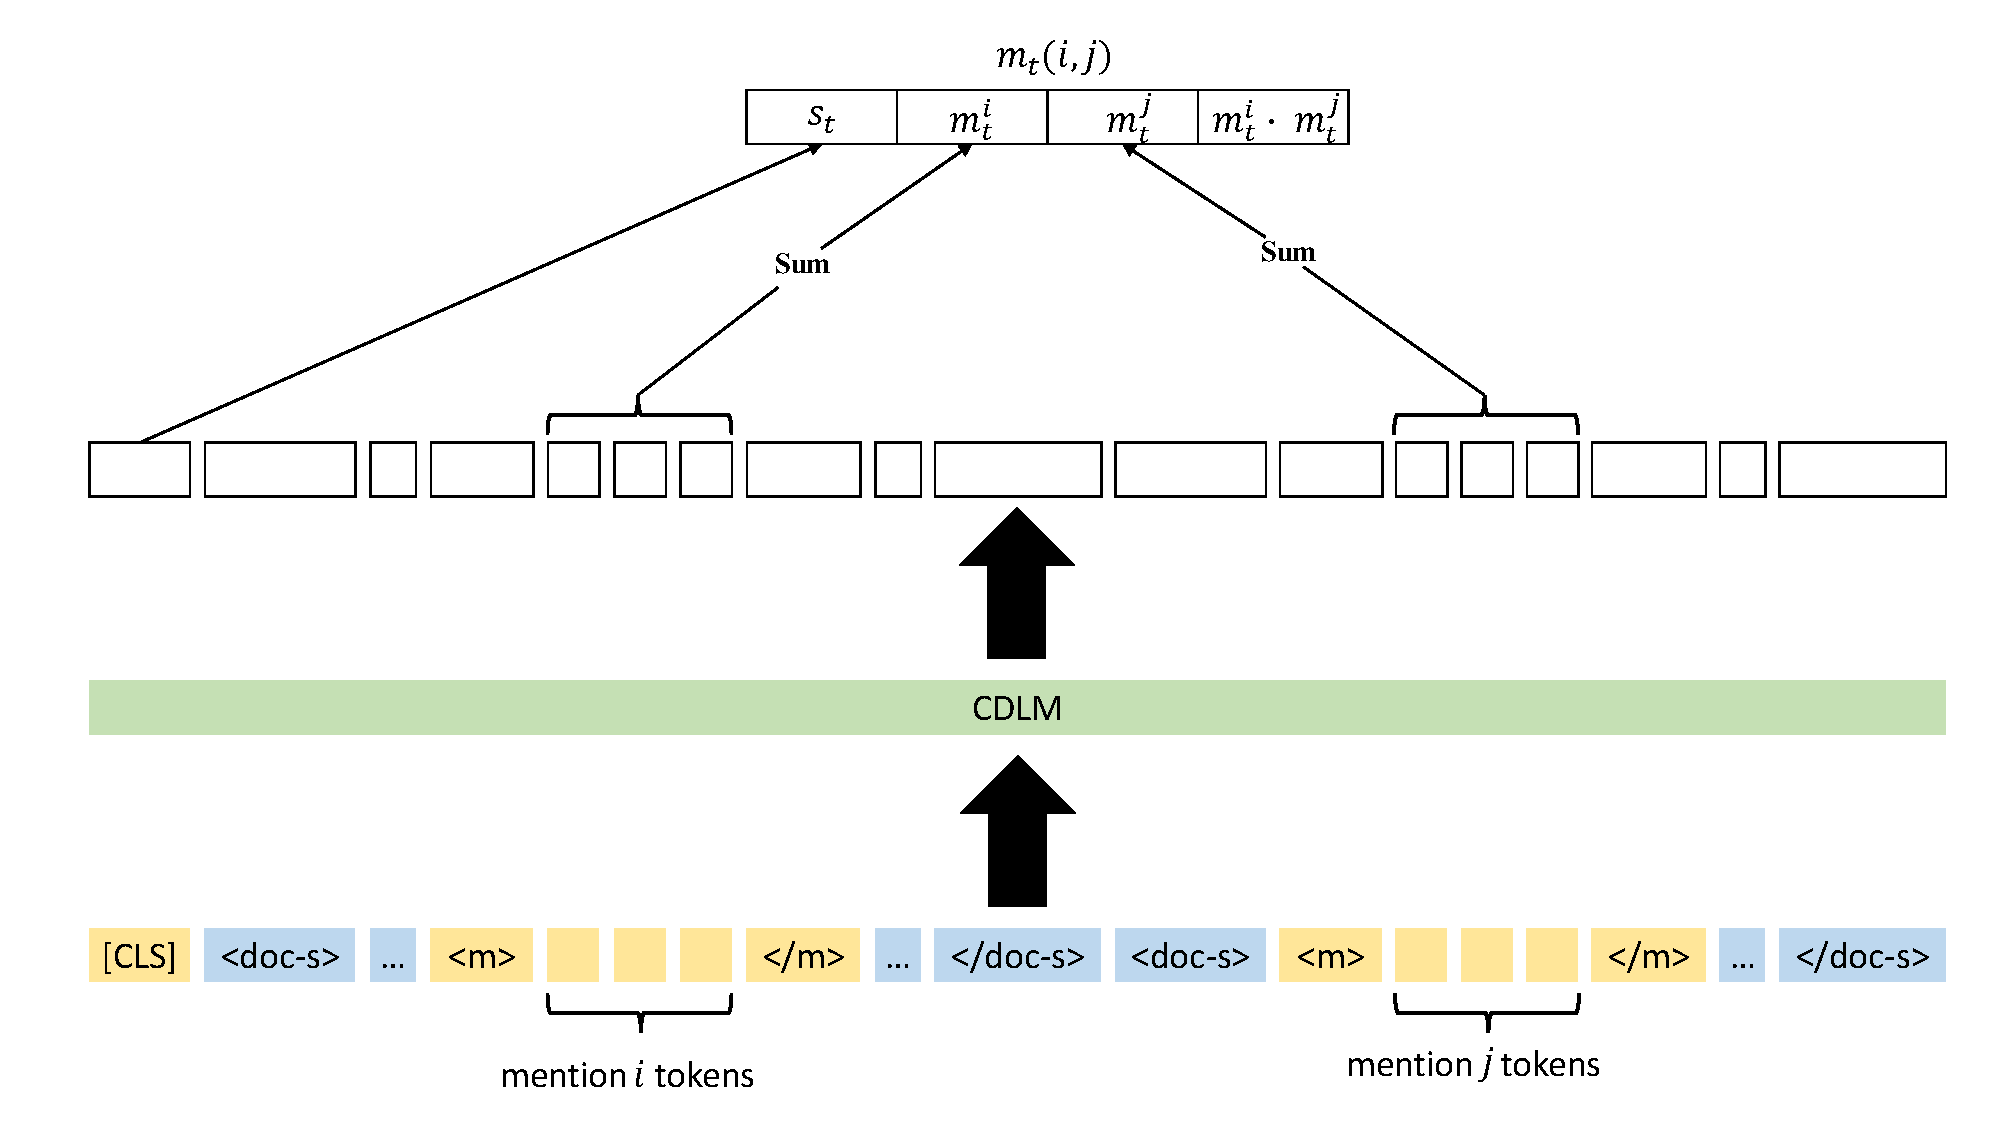
\includegraphics[width=\textwidth,height=\textwidth,keepaspectratio]{images/CDLM.pdf}
  \caption{The CDLM model utilizes pairwise mention representation for coreference resolution. $m_t^i$, $m_t^j$ and $s_t$ are the cross-document contextualized representation vectors for mentions $i$ and $j$, and of the [CLS] pairwise-mention representation. The tokens colored in yellow represent global attention, and the tokens colored in blue represent local attention.}
  \label{fig:cdlm}
\end{figure}

Upon completing coreference resolution in both single-document and cross-document scenarios, we integrate coreference relationships (:coref) into the KGs. These links signify the coreference relationships between the events and entities, aiding in the generation of claims that incorporate information from multiple documents. Figure~\ref{fig:visulization} illustrates the multimodal multi-document knowledge graph. Colors signify distinct documents, and the connection between nodes of different colors indicates coreference for a shared event or entity.


            \subsection{Knowledge Graph Completion with LLMs} \label{se:KGC_LLM}
                To uncover latent relationships within multiple documents, we utilize Vicuna~\cite{vicuna2023} for knowledge graph completion. Vicuna is a cutting-edge model designed for natural language understanding tasks. Leveraging advanced techniques, it excels in tasks such as text summarization, sentiment analysis, and language translation. Its robust architecture ensures high-performance outcomes across diverse applications.

The process involves inputting multimodal multi-document claims generated by~\textbf{KG2Claim} into Vicuna. Subsequently, prompts are employed to extract latent information from these claims. This ensures the incorporation of latent information derived from such claims. Furthermore, the completion claims are inserted into knowledge graphs to enhance available resources.

\begin{figure}
\centering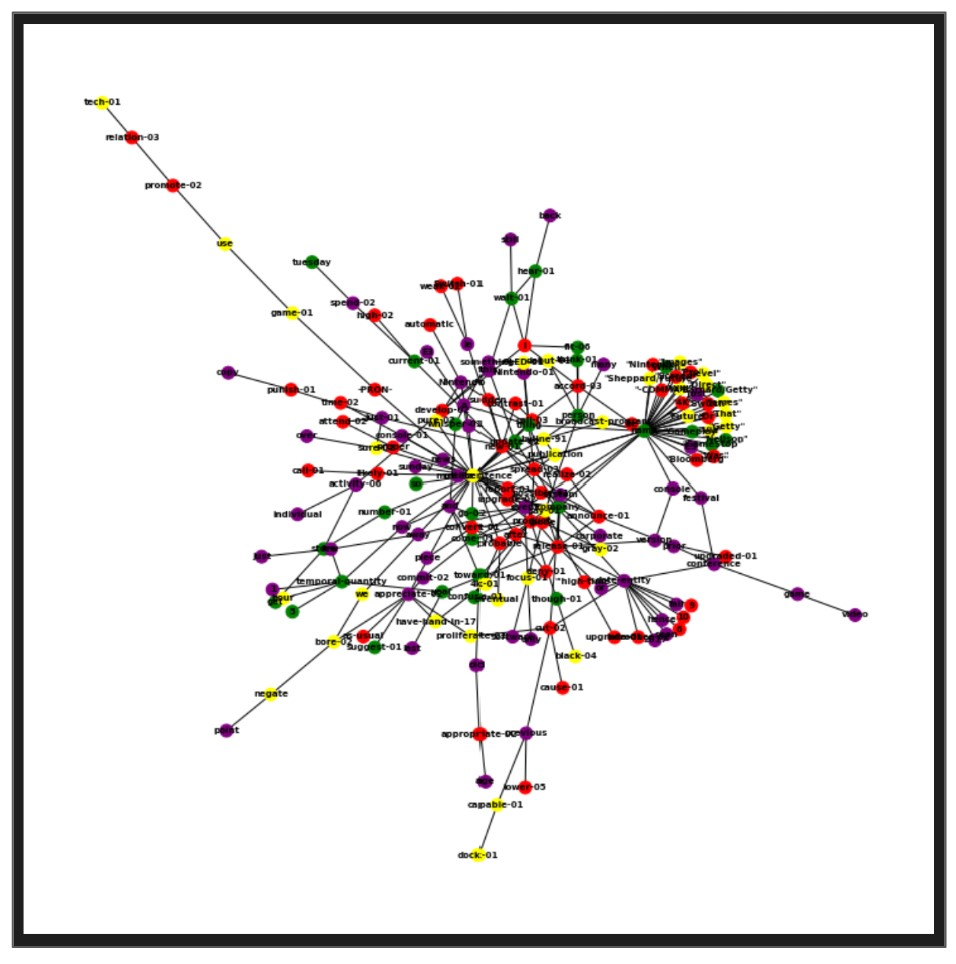
\includegraphics[width=\textwidth,height=\textwidth,keepaspectratio]{images/11.jpg}
  \caption{The knowledge graph is depicted with color-coded elements denoting multi-document sources. In our research, a maximum of four documents is utilized.}
  \label{fig:visulization}
\end{figure}
            \subsection{Knowledge-Driven Claim Generation}
            \label{se:KDCG}
                To produce multimodal multi-document claims from Knowledge Graphs (KGs), we devise a traversal method specifically tailored for KGs featuring coreference relationships (:coref). The traversal method is detailed in Algorithm~\ref{alg:one}. Additionally, we utilize the AMRBART model~\cite{bai2022graph} to generate multimodal multi-document claims based on the information extracted from the knowledge graphs. AMRBART is a BART~\cite{lewis2019bart} model pretrained on AMR graphs by introducing graph self-supervised training. AMRBART utilizes two graph auto-encoding strategies for graph-to-graph pre-training and integrating text and graph information through four tasks.

We feed the traversal results into AMRBART to generate the text. The~\textbf{KG2Claim} method is a text generation method for our detecting disinformation project. We totally generated 816,115 multimodal multi-document claims in the NewsStories dataset. This method focuses on detailing the processing of text representation and traversal algorithms involving coreference relationships.

\begin{algorithm}[H]
\caption{Traversal algorithm}\label{alg:one}
\begin{algorithmic}[1]

\State Input: Graph $G$ includes sets of (h,r,t) triple
\State Outputs: Set of triples with the coreference relationships (:coref)
\State Search all predicate nodes $\mathrm{P}$ that have :ARG relationships 
\For{$\mathrm{p} \in \mathrm{P}$}
    \State Traversal results = CorefDFS(G, p)
\EndFor

\Function{CorefDFS}{Graph, start, visited=None}
    \State visited = set()
    \State Stack=[start]
    \While {Stack}
        \State vertex = Stack.pop()
        \If {vertex not in visited}
            \State visited.append(vertex)
            \State neighbors = sort(Graph[vertex], key=:coref, reverse=True)
            \State Stack.append(neighbor for neighbor in neighbors if neighbor not in visited)
        \EndIf
    \EndWhile
    \State \Return Stack
\EndFunction 

\end{algorithmic}
\end{algorithm}
                
    \chapter{Results} \label{ch:results}

        \section{Claim Verification} \label{se:CV}
            \begin{table}[]\Large
\centering
\caption{ Performance of claim verification in MOCHEG with our method. We separately calculate the precision and recall in supported, refuted, and NEI claim labels. We compare our method with published baselines in Table~\ref{label:claim_verification_fscore_MOCHEG}.}
\resizebox{\textwidth}{!}{
\begin{tabular}{l|ccccccc}\hline
\textbf{Setting}      & \textbf{Accuracy (\%)} & \textbf{\begin{tabular}[c]{@{}c@{}}Precision (\%)\\ Supported\end{tabular}} & \textbf{\begin{tabular}[c]{@{}c@{}}Precision (\%)\\ Refuted\end{tabular}} & \textbf{\begin{tabular}[c]{@{}c@{}}Precision (\%)\\ NEI\end{tabular}} & \textbf{\begin{tabular}[c]{@{}c@{}}Recall (\%)\\ Supported\end{tabular}} & \textbf{\begin{tabular}[c]{@{}c@{}}Recall (\%)\\ Refuted\end{tabular}} & \textbf{\begin{tabular}[c]{@{}c@{}}Recall (\%)\\ NEI\end{tabular}} \\
\hline
Our w/ Text Evidence $\rightarrow$ DeBERTa V3  & 43.7 & 79.2 & 66.9 & \textbf{33.9} & 40.5 & 30.6 & 25.8\\
Our w/ Text and Image Evidence $\rightarrow$ DeBERTa V3 & 50.8 & 83.4 & \textbf{69.3} & 27.3 & 42.9 & 34.2 & 30.9\\
Our w/ Text Evidence $\rightarrow$ Llama 2  & 46.7 & 80.4 & 68.1 & 31.5 & 37.2 & 35.4 & 31.5\\
Our w/ Text and Image Evidence $\rightarrow$ Llama 2 & \textbf{53.7} & \textbf{87.3} & 60.3 & 32.4 & \textbf{48.3} & \textbf{36.9} & \textbf{34.8} \\
Our w/Text Evidence $\rightarrow$ Stance detection model & 40.5& 79.4& 68.3& 32.3& 43.7& 34.2& 14.4\\
Our w/ Text and Image Evidence $\rightarrow$ Stance detection model & 45.4& 76.8& 66.9& 34.7& 35.7& 36.2& 30.9\\
\hline
\end{tabular}}
\label{label:MOCHEG}
\end{table}

The goal of our method is to generate a summary from multiple documents and modalities that is useful for fact-checking a claim. In order to assess how useful our method is at this task, we compare the performance of our method on MOCHEG, which presents a benchmark and method for multimodal multi-document fact-checking.

Specifically, we employed three~\textit{fixed} entailment models, namely DeBERTa V3~\cite{he2023debertav3}, Llama-2-70b~\cite{touvron2023llama}, and stance detection model~\cite{Yao_2023}, as our surrogate "human" fact-checkers. The goal of these models is to predict the entailment label of a claim given our generated summary. Importantly, we do not finetune these models with our generated summaries so as to not bias the models towards linguistic or stylistic patterns of the summarizer. As depicted in Tables~\ref{label:MOCHEG} and~\ref{label:claim_verification_fscore_MOCHEG}, our method exhibits superior performance, achieving a SOTA 48.2 F-score in the MOCHEG dataset. Furthermore, according to Table~\ref{label:MOCHEG}, our method demonstrates strong precision performance for the "supported" label and strong recall performance in the "supported", "NEI", and "refuted" labels.


\begin{table}[!th]\large
\centering
\caption{Performance of claim verification in MOCHEG. DeBERTa V3, Llama-2-70b, and the stance detection model represent the fixed entailment models. Gold Evidence denotes ground truth text and image evidence while System Evidence means automatically retrieved text and image evidence.}
\begin{tabular}{l|c}
\hline
\textbf{Setting}                       & \textbf{F-score (\%)} \\ \hline
Our w/ Text Evidence $\rightarrow$ DeBERTa V3           & 42.7                   \\
Our w/ Text and Image Evidence $\rightarrow$ DeBERTa V3 & 45.1                   \\
Our w/ Text Evidence $\rightarrow$ Llama 2           & 43.9                 \\
Our w/ Text and Image Evidence $\rightarrow$ Llama 2 & \textbf{48.2}                   \\
Our w/Text Evidence $\rightarrow$ Stance detection model & 41.8\\
Our w/ Text and Image Evidence $\rightarrow$ Stance detection model & 43.3\\
\hline
MOCHEG w/ Text Evidence                 & 42.7                \\
MOCHEG w/ Image Evidence                & 40.9                \\
MOCHEG w/ Text and Image Evidence       & \textbf{44.0}                \\ \hline
Human w/o Evidence                      & 20.0                \\
Human w/ System Evidence                & 62.0                \\
Human w/ Gold Evidence                  & \textbf{70.0}                \\ \hline
\end{tabular}
\label{label:claim_verification_fscore_MOCHEG}
\end{table}

Table~\ref{label:MOCHEG} reveals that the best results are achieved when inputs incorporate both textual and image evidence. Perhaps unsurprisingly given its size, the zero-shot Llama-2-70b entailment surrogate model surpasses DeBERTa V3 in performance. Nevertheless, a notable issue persists, where the surrogate entailment models struggle to accurately deal with NEI claim labels.

Table~\ref{label:claim_verification_fscore_MOCHEG} highlights the superiority of our model compared to MOCHEG. In the case of MOCHEG, truthfulness labels are predicted by averaging a stance representation derived from both textual and image evidence. Furthermore, MOCHEG's classifier relies on fixed thresholds, which may not be optimal for every situation. In contrast, our approach involves generating summaries for fact-checking via reinforcement learning with fixed entailment models. Although a difference remains in the result of human vs system prediction performance, our model surpasses the prior state-of-the-art system by 4.2\% F-score.


        \section{Explanation Generation} \label{se:EG}
            \begin{table}[th]\Large
\centering
\caption{Performace of explanation generation. Our system outperforms MOCHEG on equivalent settings. Gold Evidence denotes ground truth text and image evidence while System Evidence means automatically retrieved text and image evidence. Gold Truthfulness denotes ground truth truthfulness label while System Truthfulness means the predicted truthfulness label.}
\resizebox{\textwidth}{!}{
\begin{tabular}{l|cccccc}
\hline
\textbf{Setting} & \textbf{ROUGE 1 (\%)} & \textbf{ROUGE 2 (\%)} & \textbf{ROUGE L (\%)} & \textbf{BLEU (\%)} & \textbf{BERTScore (\%)}\\ \hline
MOCHEG w/ Gold Evidence, Gold Truthfulness      & \textbf{45.5}   & \textbf{27.3}   & \textbf{35.4}   & \textbf{21.8}   & \textbf{89.0}   \\
MOCHEG w/ Gold Evidence, System Truthfulness    & 43.8   & 26.3   & 34.1   & 20.8   & 88.8   \\
MOCHEG w/ System Evidence, Gold Truthfulness    & 35.5   & 17.4   & \textbf{26.0}   & \textbf{10.9}   & 87.0   \\
MOCHEG w/ System Evidence, System Truthfulness  & 33.8   & 16.5   & 24.8   & 10.0   & 86.9   \\
Our w/ System Evidence, Gold Truthfulness      & \textbf{36.7}   & \textbf{17.9}   & 25.7   & 10.7   & \textbf{87.3}  \\
Our w/ System Evidence, System Truthfulness    & 34.3   & 16.8   & 25.4   & 10.4   & 87.1  \\\hline
\end{tabular}}
\label{label:explanation_generation}
\end{table}

In order to assess the degree to which our generated summaries contain the relevant facts necessary to fact-check the generated claims, we measure the ability of a method to generate an~\textit{explanation} of the predicted truthfulness label using our summary. We adopt a methodology similar to~\citet{Yao_2023}, where we consider the input claim $C$, its truthfulness label $Y_C$, and the summary for fact-checking $\{T_1, T_2, ...\}$ generated from~\textbf{MetaSumPerceiver}.  These components are concatenated into an overall sequence $X$ using a separator </s>. During the training of the rationale generator, We employ the actual truthfulness label of each claim as input. Critically, we do not retrain or fine-tune~\textbf{MetaSumPerceiver} for this task. In the evaluation phase, we utilize the truthfulness label predicted by the fixed entailment models. Following~\citet{Yao_2023}, we utilize BART based to generate the ruling statement. Our evaluation metrics include ROUGE~\cite{lin-2004-rouge}, BLEU~\cite{10.3115/1073083.1073135}, and Bertscore~\cite{zhang2020bertscore}. To assess the performance of explanation generation, we compare it with MOCHEG~\cite{Yao_2023}, as shown in Table~\ref{label:explanation_generation}.

\begin{figure*}[th]
  \centering
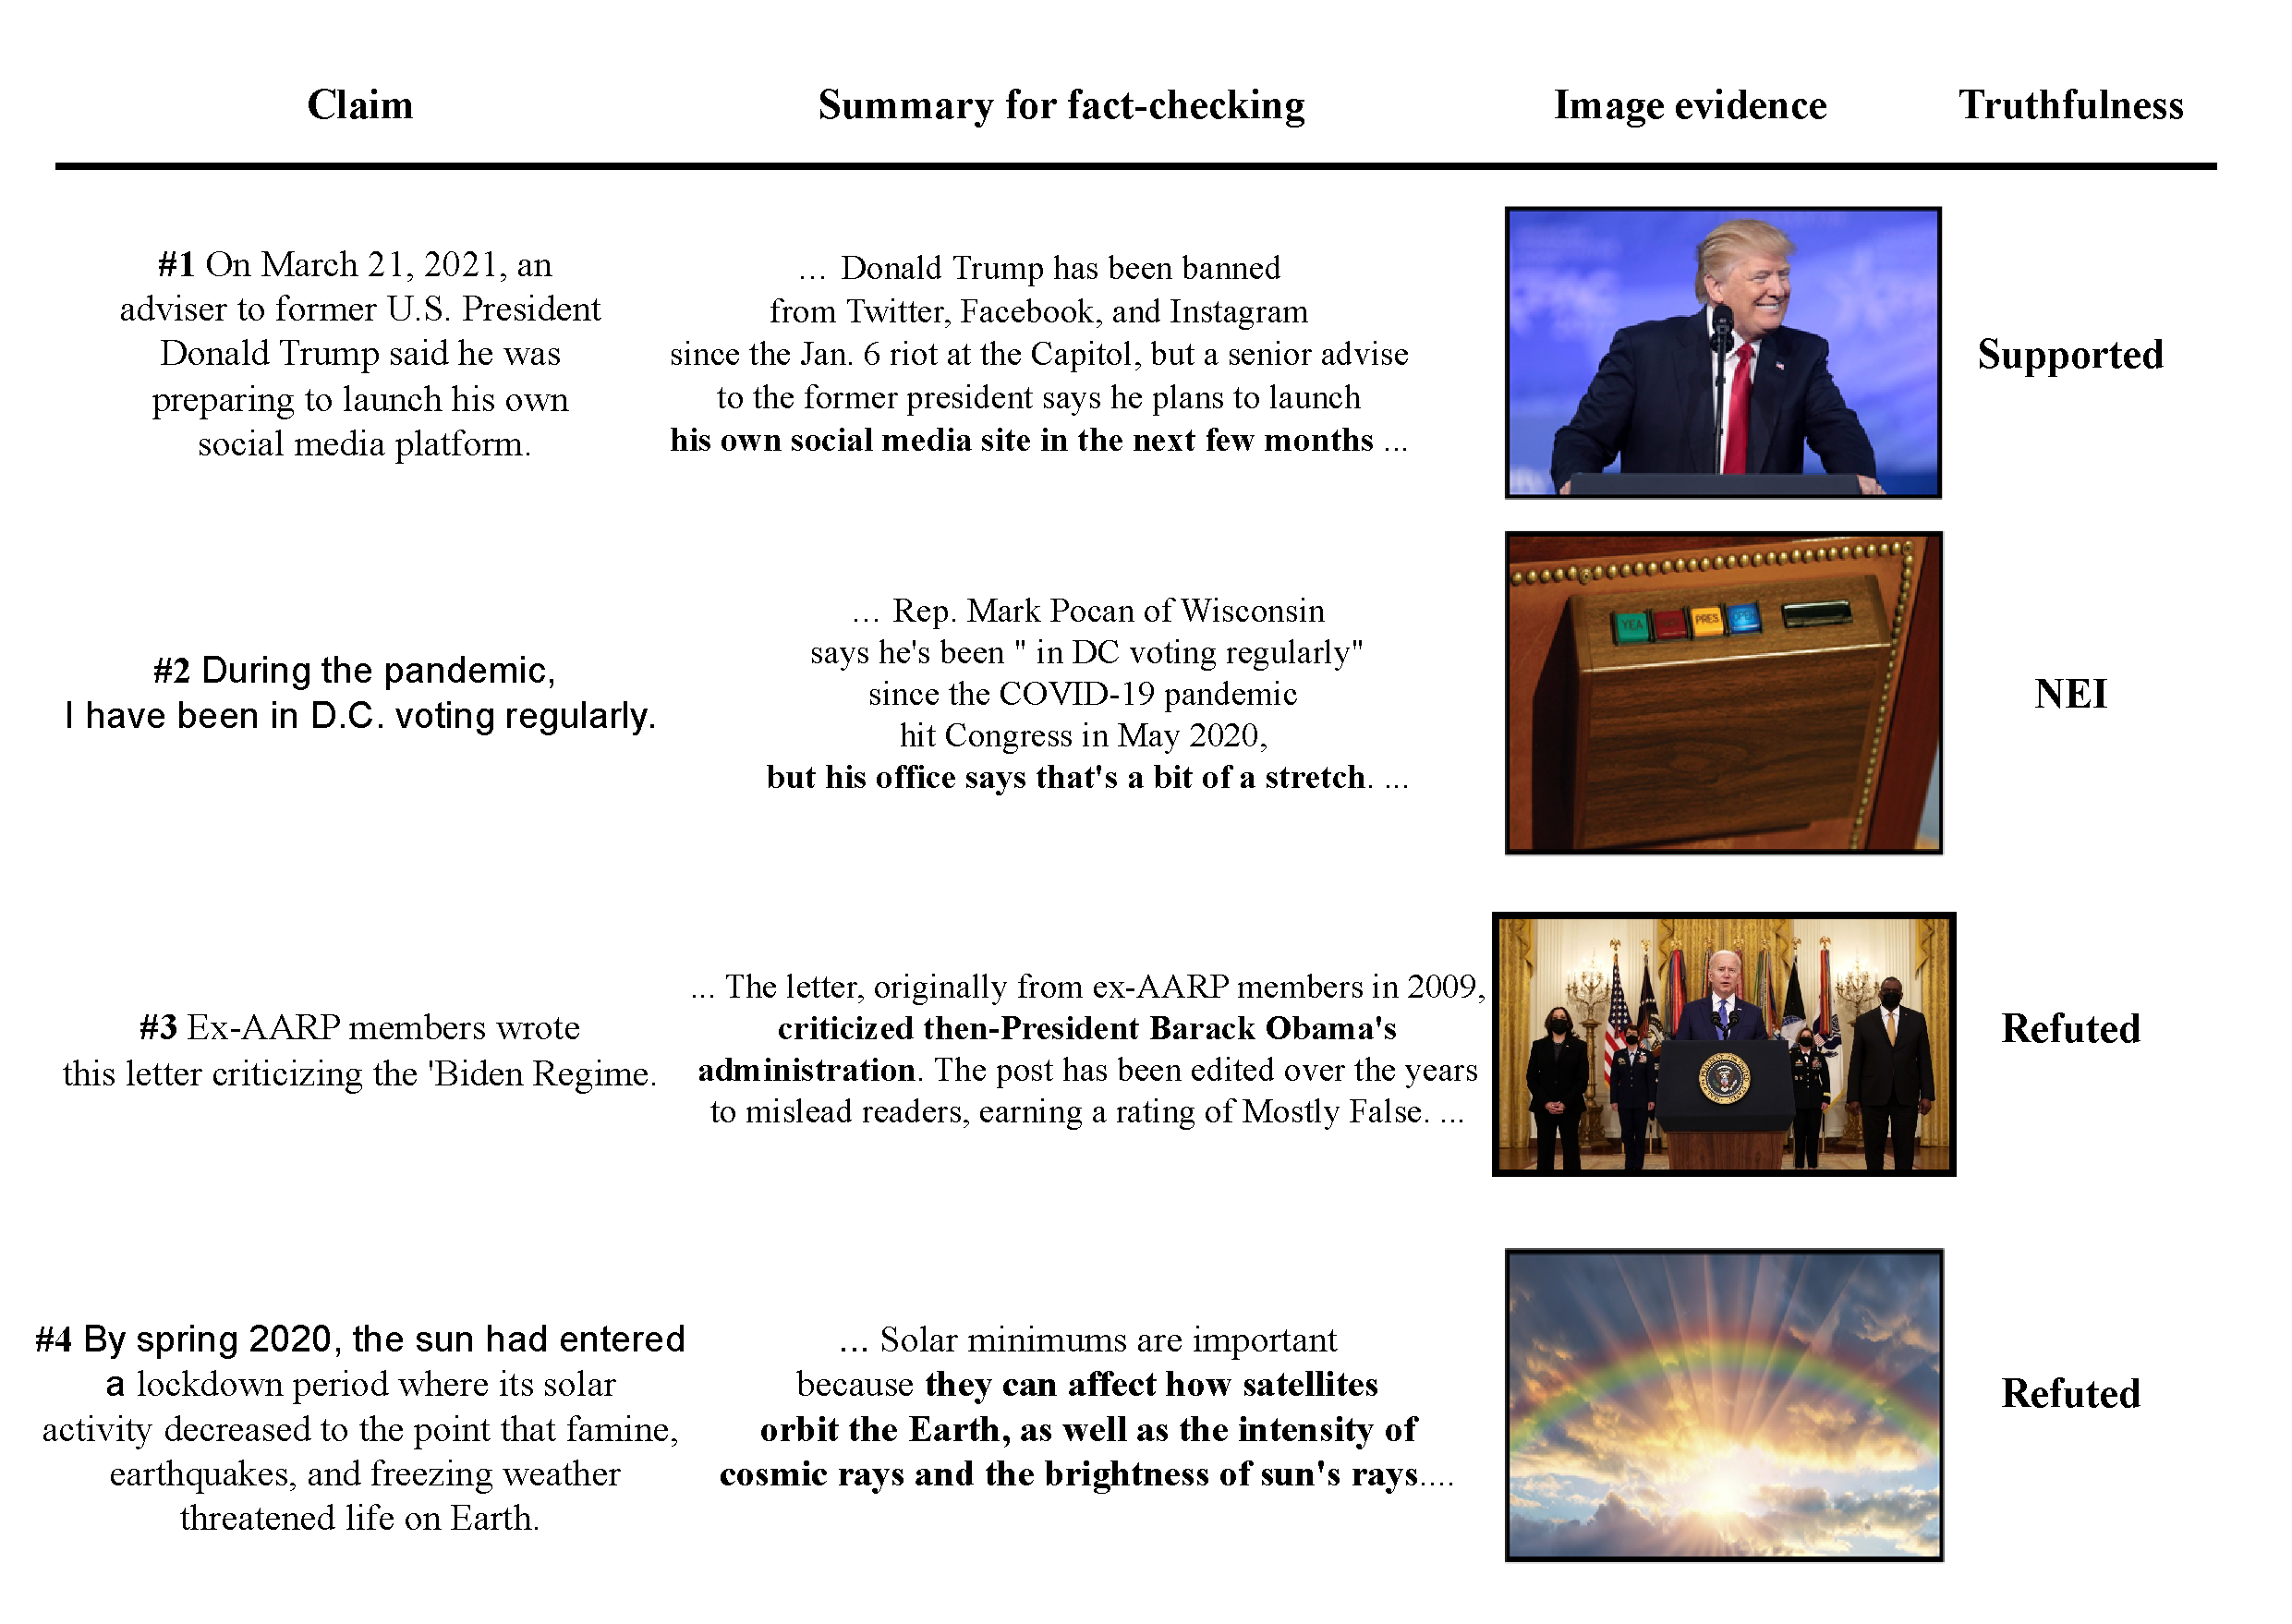
\includegraphics[width=\textwidth,height=\textwidth,keepaspectratio]{images/multimodal-fact-checking.pdf}
  \caption{Evidence summary examples in the explanation generation task. The truthfulness column shows gold labels. For instance, the third claim's article primarily discusses a letter critiquing the Obama administration. However, given President Joe's past collaboration with Ex-President Obama, the letter was manipulated to criticize the 'Biden Regime.' This assertion lacks support from credible sources, making it a refuted claim.}
  \label{fig:qualitative}
\end{figure*}

We observe that our model outperforms MOCHEG's evidence-retrieval-based method ("system evidence") on the rationale generation task. In our case, "system evidence" is our generated summary. We note that MOCHEG's method relies on retrieval from a pool of multimodal documents. The ground truth explanations rely on these sentences and thus may share some phrasing. This gives a slight advantage to MOCHEG's method on some metrics that measure n-gram overlap, whereas our method based on summarization may rephrase the same evidence. Nevertheless, we observe that our system outperforms MOCHEG's generated explanations. We further observe that our explanations generated using system evidence and system truthfulness outperform MOCHEG's method, which relies on the ground truth truthfulness label on the BERTScore metric. Overall, these results demonstrate that our summarizer, which was not trained for the rationale prediction task, is capturing relevant evidence across modalities in a short summary better than MOCHEG's evidence retrieval-based approach.

We illustrate our generated summaries for fact-checking in Figure~\ref{fig:qualitative}. Our results show that our summaries contain sufficient evidence to determine the accuracy of the claim label. Whether the truthfulness label is supported, labeled as NEI (No Evidence Identified), or refuted, we consistently provide evidence for a fact-checker to make a determination of the truthfulness of the claim.

\begin{table}[h]\Large
\centering
\caption{Evaluating the effectiveness of our multimodal multi-document claims using the pre-trained claim detection model.}
\begin{tabular}{l|c}
\hline
\textbf{Claim classes}                    & \textbf{Category percentage(\%)}  \\\hline
Unimportant Factual Sentence (UFS)        & 17.67          \\
Check-worthy Factual Sentence (CFS)       & 68.6           \\
Non-factual Sentence (NFS)                & 13.71          \\\hline
\end{tabular}
\label{label:claim_detect}
\end{table}

        \section{Multimodal Multi-document Claims Analysis} \label{se:MMCA}
            To assess the effectiveness of~\textbf{KG2Claim}, we evaluate the generated claims with the check-worthy classification task. In Table~\ref{label:claim_detect}, 68.6\% of the sentences identified as check-worthy factual sentences (CFS) originate from our approach. This suggests that our generated claims encompass factual information that the general public would find interesting and worth verifying. Additionally, 17.67\% of sentences in our dataset are factual but deemed unimportant for fact-checking (UFS), indicating a lack of public interest in these claims. Finally, 13.71\% of sentences in our data are non-factual (NFS), primarily comprising questions, beliefs, and declarations. 

The results reveal two main points. Firstly, we effectively integrate multimodal multi-document sources, as over 60\% of our generated claims focus on public interest. This indicates that our traversal algorithm is well-suited for knowledge graphs. Secondly, the content of our generated claims is closely tied to the US election in the ClaimBuster dataset~\cite{arslan2020benchmark}, specifically in the policy domain rather than other areas.

\begin{table}[h]\Large
\centering
\caption{Performance of detecting truthfulness label in Multimodal Multi-document claims.}
\begin{tabular}{l|c}
\hline
\textbf{Truthfulness labels}                    & \textbf{Category percentage(\%)}  \\\hline
Entailment label &  74.3  \\
Neutral label &   8.24     \\
Contradiction label &  17.46 \\\hline
\end{tabular}
\label{label:claim_label}
\end{table}
        \section{Multimodal Multi-document Claims Truthfulness Label Test}
        \label{se:MMCT-Per}
            In our assumption, we consider the multimodal multi-document claims to be entirely entailed with news articles, images, and videos, as these claims are generated from multimodal knowledge graphs. To verify this assumption, we tested the generated claims using our~\textbf{MetaSumPerceiver} model. When the claim and multimodal multi-document sources are provided to the model, it determines whether the claim is entailed by the news using the entailment model. In Table~\ref{label:claim_label}, 74.3\% of our claims are confirmed to be entailed with news articles, indicating a definite connection with the sources. Additionally, 8.24\% of our claims are categorized as neutral, meaning that the content does not contradict the news, but further consideration is needed to determine the accuracy of the relationships in these claims. Finally, 17.46\% of our claims are contradiction claims, clearly indicating that these claims are unrelated to the news. The reason behind this is that the content of these claims revolves around advertisements in news articles.

The results provide insights that differ from our initial assumption. We suspect that the discrepancy may arise from the edge labels in the knowledge graphs. We believe it's essential to introduce additional edge labels to categorize less important information. This approach would help us steer clear of certain edges and nodes during the traversal of knowledge graphs.

\begin{table}[h]\Large
\centering
\caption{Accuracy for prompting entailment, neutral, contradiction claims with Llama-2-70b in Multi-News-Fact-Checking dataset.}
\begin{tabular}{l|c}
\hline
\textbf{Claims}      & \textbf{Accuracy(\%)} \\ \hline
Entailment claims    & 78.3          \\
Nentral claims       & 64.2          \\
Contradiction claims & 74.1          \\ \hline
\end{tabular}
\label{label:prompt_accuracy}
\end{table}
        \section{Refining Multi-News-Fact-Checking Dataset} \label{se:RMNFCD}
            In section~\ref{subse:MNFCD}, we described how we generated the claims and labels comprising our Multi-News-Fact-checking dataset. In total, our dataset consists of 1,687,200 claims and labels. However, in some cases, Llama-2-70b misunderstands the summary and predicts the wrong label for the claims. To assess the quality of our dataset, we employ Llama-2-70b once again for a thorough validation of our dataset's claims and respective labels (entailment, neutral, and contradiction). We provide the prompt we use for this double-checking procedure in the appendices~\ref{ase:app_prompt_llama2} and show the prompted claims in Figure~\ref{fig:prompt_ex}.

In Table~\ref{label:prompt_accuracy}, we show the performance of Llama-2-70b at predicting the label produced from the first phase of our dataset. We show that Llama-2-70b exhibits strong performance on entailment claims (acc 78.3\%) and contradiction claims (acc 74.1\%). We observe that Llama-2-70b performs worse at distinguishing neutral claims, registering an accuracy of only 64.2\%. This is likely because the neutral category requires identifying that a specific piece of a claim is neither entailed or contradicted. Thus, this case is harder than either entailment or contradiction alone. We show examples of specific prompts and corresponding entailment, neutral, and contradictory claims.

Additionally, we discovered that most predictions from Llama-2-70b are similar to human predictions, especially in entailment and contradiction claims. To investigate this similarity further, we conducted a human test by randomly selecting 200 claims. The results for entailment claims revealed that 65\% of them had the same prediction as Llama-2-70b. For contradiction claims, 73\% of the sampled claims matched Llama-2-70b's predictions. Finally, in neutral claims, 62\% of the sampled claims had the same prediction as Llama-2-70b.

\begin{table}[]\large
\centering
\caption{Performance of claim verification in Multi-News-Fact-Checking dataset. We compare our method with other offline summarization models.}
\resizebox{\textwidth}{!}{
\begin{tabular}{l|cccccccc}\hline
\textbf{Setting}      & \textbf{Accuracy (\%)} & \textbf{\begin{tabular}[c]{@{}c@{}}Precision (\%)\\ Entailment \end{tabular}} & \textbf{\begin{tabular}[c]{@{}c@{}}Precision (\%)\\ Contradiction\end{tabular}} & \textbf{\begin{tabular}[c]{@{}c@{}}Precision (\%)\\ Neutral\end{tabular}} & \textbf{\begin{tabular}[c]{@{}c@{}}Recall (\%)\\ Entailment\end{tabular}} & \textbf{\begin{tabular}[c]{@{}c@{}}Recall (\%)\\ Contradiction\end{tabular}} & \textbf{\begin{tabular}[c]{@{}c@{}}Recall (\%)\\ Neutral\end{tabular}} \\
\hline
PEGASUS $\rightarrow$ DeBERTa V3 & 33.2 & 64.2& 14.7& 21.5& 37.3& 12.4& 11.9 \\
PEGASUS $\rightarrow$ Llama 2 & 39.5 & 37.4& 23.1& 42.8& 27.6& 24.3& 24.0\\ \hline
T5 large $\rightarrow$ DeBERTa V3 & 34.8 & 62.8& 17.5& 26.2& 33.0& 18.5& 18.2\\
T5 large $\rightarrow$ Llama 2 & 37.2 & 40.2& 32.8& \textbf{48.0}& 30.5& 26.4& 26.8\\ \hline
Our $\rightarrow$ DeBERTa V3 & 36.7 & \textbf{75.5} & 28.9 & 27.5 & 41.0 & 21.7 & \textbf{47.2} \\
Our (No RL) $\rightarrow$ Llama 2 & 42.6 & 41.0 & \textbf{53.7} & 34.6 & 54.8 & 37.8 & 29.6 \\ 
Our $\rightarrow$ Llama 2 & \textbf{45.6} & 49.2 & 48.7 & 33.6 & \textbf{56.9} & \textbf{44.1} & 28.4 \\ \hline
\end{tabular}}
\label{label:multi-news}
\end{table}
        \section{Ablation} \label{se:ablation}
            Additionally, we conducted ablation experiments for claim verification on our Multi-News-Fact-Checking dataset. A comparative analysis of our method with Llama-2-70b and other offline summarization models, PEGASUS~\cite{zhang2020pegasus} and T5 large~\cite{2020t5}, is presented in Tables~\ref{label:multi-news_fscore} and~\ref{label:multi-news}.

Similar to our results in MOCHEG, Tables~\ref{label:multi-news_fscore} and~\ref{label:multi-news} show that our approach, when employing the Llama-2 surrogate entailment model, achieves the best performance. Furthermore, we achieve balanced accuracy in both precision and recall, underscoring our method's ability to clearly differentiate between truthful and untruthful labels without bias in predictions. The results highlight the inability of other summarization models to generate summaries useful for fact-checking, which causes the surrogate model difficulty in accurately assessing the truthfulness labels.

We also established human performance upper bounds on our Multi-News-Fact-Checking dataset following MOCHEG's methodology. We randomly sampled 200 claims and assigned labels for their truthfulness based on gold evidence (the human written summaries from which the claims were generated), system evidence (our generated summaries), and no evidence, resulting in F-scores of 0.76, 0.65, and 0.23, respectively.

\begin{table}[h]\small
\centering
\caption{Performance of claim verification in Multi-News-Fact-Checking dataset. DeBERTa V3 and Llama-2-70b serve as the fixed entailment models. Gold Evidence refers to claim labels based on gold standards, whereas System Evidence indicates our predicted claim labels.}
\begin{tabular}{l|c}
\hline
\textbf{Setting}             & \textbf{F-score (\%)} \\\hline
Our w/ DeBERTa V3               & 39.9                 \\
Our w/ Llama 2               & \textbf{43.4}        \\
Our w/ Llama 2(No RL)               & 41.8            \\\hline
PEGASUS w/ DeBERTa V3           & 25.4                 \\
PEGASUS w/ Llama 2           & \textbf{30.8}            \\\hline
T5 large w/ DeBERTa V3          & 28.5            \\
T5 large w/ Llama 2          & \textbf{32.7}            \\\hline
Human w/o Evidence           & 23.0            \\
Human w/ System Evidence     & 65.0               \\
Human w/ Gold Evidence       & \textbf{76.0}               \\ \hline
\end{tabular}
\label{label:multi-news_fscore}
\end{table}



            
    \chapter{Discussion} \label{ch:discussion}
        Given the societal importance of fact-checking applications, it is important that the limitations of our methods be explored. Our experimental results reveal that the surrogate entailment model often assigns truthfulness labels for entailment even when it struggles to fully grasp the relationship between the claim and the summary with evidence. This issue not only impacts the judgment of the claim label but also affects~\textbf{MetaSumPerceiver} during training. One potential solution is using a textual entailment model adept at managing this uncertainty or excluding such instances during training. Furthermore, the experimental outcomes from the~\textbf{KG2Claim} method reveal that 30\% of the generated claims are not entailed with the news sources. The challenge lies in the possibility that multimodal multi-document knowledge graphs might incorporate irrelevant information. A potential remedy is to diversify the set of edge labels in the knowledge graphs. We propose incorporating additional labels, such as the content label, ads label, and quote label. This approach would help prioritize which edges are more crucial for traversal. Lastly, Llama 2's claims in the Multi-News-Fact-Checking dataset have certain flaws. Our review suggests that neutral claims might mix consistent and conflicting details. Enhancing our data creation prompts or the prompts used in the second-stage claiming could boost Llama 2's understanding.

~\textbf{MetaSumPerceiver}, trained on English text and topics from the Multi-News benchmarks, may not perform well in other languages without retraining. Care should be taken to ensure the model is trained on data that closely aligns with the target domain of interest, if possible, to minimize errors. Finally, our model relies on identifying relevant and trusted source documents on which to perform summarization and checking. While this document-level retrieval task is orthogonal to our research, failure to retrieve relevant documents will affect the downstream performance of the fact-checking system. If irrelevant documents are used, even true claims might be wrongly challenged. Thus, approaches should confirm that events and entities in sourced documents are directly related, employing sophisticated methods.

        
    \chapter{Conclusions} \label{ch:conclusions}
        We introduce~\textbf{MetaSumPerceiver}, a summarization model designed to produce concise, informative summaries for claim fact-checking from complex multimodal datasets. Our model's flexible architecture can accommodate arbitrary numbers of documents and types of inputs, including documents, images, and claims by leveraging a perceiver-based architecture. In addition, we propose~\textbf{KG2Claim}, a text generation pipeline to produce the claims from the knowledge graphs. Our text generation approach can generate claims related to multimodal mult-document information.

We train our model using a novel reinforcement learning approach in order to generate summaries useful for verifying the truthfulness of claims. Our experimental assessments on the MOCHEG and our Multi-News-Fact-Checking datasets highlight~\textbf{MetaSumPerceiver}'s robust performance in claim verification tasks and demonstrate its effectiveness in real-world fact-checking scenarios. This contribution underscores ~\textbf{MetaSumPerceiver}'s potential to streamline fact-checking processes in today's multimodal information landscape. Moreover, we release the publicly accessible Multi-News-Fact-Checking dataset, aimed at assisting researchers in developing multi-document fact-checking methods.

Furthermore, we employ our text generation pipeline to produce claims in the NewsStories dataset. Our analysis of the generated claims reveals that more than 60\% are factual, drawing public interest in fact-checking. Additionally, testing these claims with~\textbf{MetaSumPerceiver} demonstrates that over 70\% of them are entailed with the news sources. According to the above experiment, the conclusion indicates that more than 60\% of the claims are entailment claims, and people wish to discern whether they are correct.

	% This is the standard bibtex file. Do not include the .bib extension in <bib_file_name>.
	% Uncomment the following lines to include your bibliography: 
	\bibliography{bib}
    \bibliographystyle{unsrtnat}
	%\bibliographystyle{unsrt}%plainnat

	% This formats the chapter name to appendix to properly define the headers:
	\appendix

	% Add your appendices here. You must leave the appendices enclosed in the appendices environment in order for the table of contents to be correct.
	\begin{appendices}
		\chapter{Prompting Design} \label{app:prompt}
			\section{Multi-document Generated and Checked Prompts} \label{ase:app_prompt_llama2}
                In the chapter~\ref{subse:MNFCD} and~\ref{se:RMNFCD}, I reference the prompts for generating and checking in the provided information:

\begin{itemize}
    \item \textbf{Entailment claim}: Task: You will be provided with a summary of a news article. Your goal is to generate a list of statements derived from the summary. These statements should be definitively true based solely on the information in the summary. Example summary: The unemployment rate dropped to 8.2\% last month, but the economy only added 120,000 jobs, when 203,000 new jobs had been predicted, according to today's jobs report. Reaction on the Wall Street Journal's MarketBeat Blog was swift: "Woah!!! Bad number." The unemployment rate, however, is better news; it had been expected to hold steady at 8.3\%. But the AP notes that the dip is mostly due to more Americans giving up on seeking employment. You will be given a summary of a news article. Your job is to generate a list of entailment claims(true) from the summary. For example, if the summary says job growth was expected to be 100,000 jobs, but only was 80,000 jobs, one simple claim you might write could be "Job growth missed expectations." Please write a numbered list of 10 claims from this summary (numbered 1. through 10.).
    \item \textbf{Neutral claim}: Task: You will be provided with a summary of a news article. Your goal is to generate a list of statements derived from the summary. These statements should not be definitively true or false based solely on the information in the summary. In other words, they should be ambiguous and require further investigation or context to determine their accuracy. Example: If the summary mentions that two celebrities are planning to get divorced, you might create a statement suggesting that their divorce might lead to significant financial and legal complications, assuming this information is not explicitly confirmed or denied in the article. Instructions: Review the provided summary. Create 10 statements based on the information in the summary. Each statement should be carefully crafted to be neither definitively true nor false based solely on the summary. Ensure that the truth or falsehood of these statements cannot be logically deduced from the summary alone. Avoid simply rephrasing or restating sentences from the summary; strive for creativity in your statement generation process. Avoid claims using statements like "may" or "could" - your claim should state things as a fact.
    \item \textbf{Contradiction claim}: Task: You will be provided with a summary of a news article. Your goal is to generate a list of statements derived from the summary. These statements should be definitively false based solely on the information in the summary. Example: If the summary mentions that a black race car starts up in front of a crowd of people., you might create a statement suggesting that a man is driving down a lonely road assuming this information is explicitly denied in the article. Instructions: Review the provided summary. Create 10 statements based on the information in the summary. Each statement should be carefully crafted to be definitively false based solely on the summary. Avoid simply rephrasing or restating sentences from the summary; strive for creativity in your statement generation process. Avoid claims using statements like "may" or "could" - your claim should state things as a contradiction fact.
    \item  \textbf{Double check claim}: Task: You will be presented with a set of documents and one claim. Your objective is to discern the claim label based on the information in the documents. The claim labels include entailment, neutral, and contradiction. Entailment signifies that the claim is conclusively true based solely on the documents. The neutral label indicates that the claim should neither be true nor false based on the information provided. The contradiction label implies that the claim is entirely false based on the information presented in the documents.
\end{itemize}

\begin{figure*}
    \hspace{-1.7cm}
    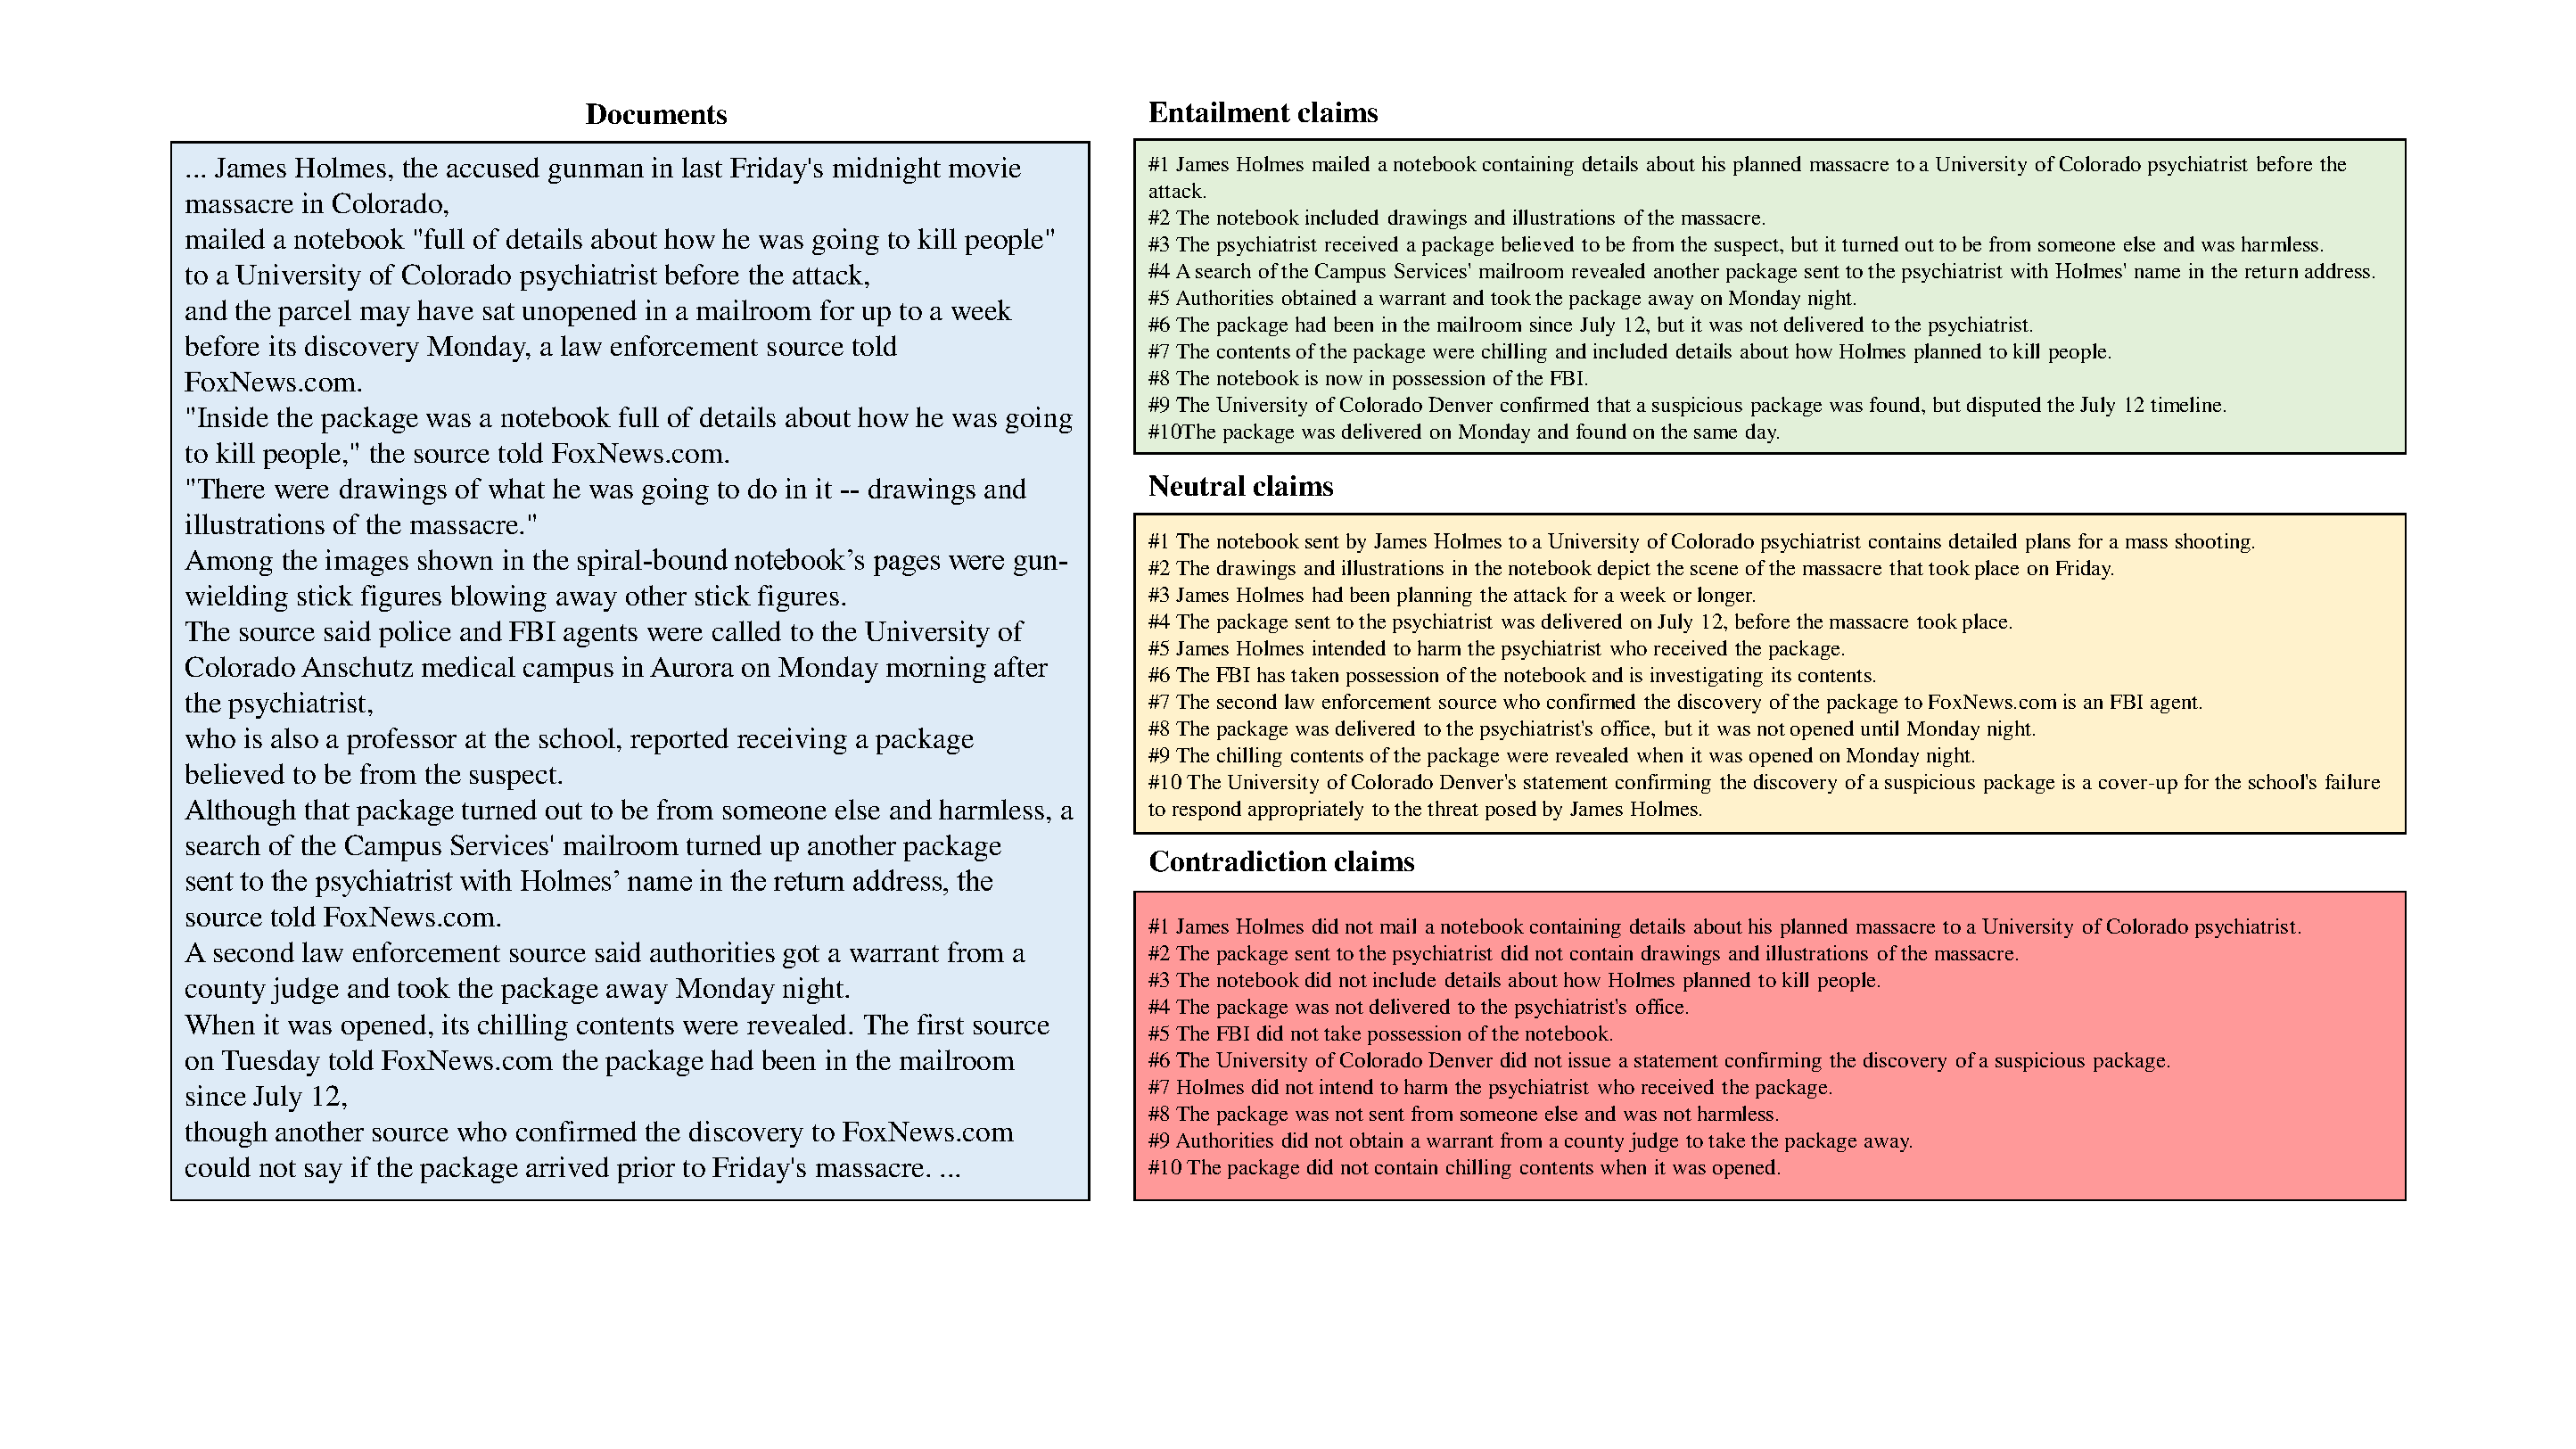
\includegraphics[width=1.2\textwidth,height=0.6\textwidth]{images/app1.pdf}
  \caption{The prompted entailment, neutral, contradiction claims from Llama-2-70b.}
  \label{fig:prompt_ex}
\end{figure*}
%				\lipsum[1-3]
%			\section{Section two} \label{ase:app_one_sect_2}
%				\lipsum[1-3]
%		\chapter{Second Appendix} \label{app:appendix_two}
%			\lipsum[2]
	\end{appendices}

\end{document}


%****************************************************************************
% Below are some general suggestions for writing your dissertation:
%
% 1. Label everything with a meaningful prefix so that you
%    can refer back to sections, tables, figures, equations, etc.
%    Usage \label{<prefix>:<label_name>} where some suggested
%    prefixes are:
%			ch: Chapter
%     		se: Section
%     		ss: Subsection
%     		sss: Sub-subsection
%			app: Appendix
%     		ase: Appendix section
%     		tab: Tables
%     		fig: Figures
%     		sfig: Sub-figures
%     		eq: Equations
%
% 2. The VTthesis class provides for natbib citations. You should upload
%	 one or more *.bib bibtex files. Suppose you have two bib files: some_refs.bib and 
%    other_refs.bib.  Then your bibliography line to include them
%    will be:
%      \bibliography{some_refs, other_refs}
%    where multiple files are separated by commas. In the body of 
%    your work, you can cite your references using natbib citations.
%    Examples:
%      Citation                     Output
%      -------------------------------------------------------
%      \cite{doe_title_2016}        [18]
%      \citet{doe_title_2016}       Doe et al. [18]
%      \citet*{doe_title_2016}      Doe, Jones, and Smith [18]
%
%    For a complete list of options, see
%      https://www.ctan.org/pkg/natbib?lang=en
%
% 3. Here is a sample table. Notice that the caption is centered at the top. Also
%    notice that we use booktabs formatting. You should not use vertical lines
%    in your tables.
% 
%				\begin{table}[htb]
%					\centering
%					\caption{Approximate computation times in hh:mm:ss for full order 						versus reduced order models.}
%					\begin{tabular}{ccc}
%						\toprule
%						& \multicolumn{2}{c}{Computation Time}\\
%						\cmidrule(r){2-3}
%						$\overline{U}_{in}$ m/s & Full Model & ROM \\
%						\midrule
%						0.90 & 2:00:00 & 2:08:00\\
%						0.88 & 2:00:00 & 0:00:03\\
%						0.92 & 2:00:00 & 0:00:03\\
%						\midrule
%						Total & 6:00:00 & 2:08:06\\
%						\bottomrule
%					\end{tabular}
%					\label{tab:time_rom}
%				\end{table}
% 
% 4. Below are some sample figures. Notice the caption is centered below the
%    figure.
%    a. Single centered figure:
%					\begin{figure}[htb]
%						\centering
%						\includegraphics[scale=0.5]{my_figure.eps}
%						\caption{Average outlet velocity magnitude given an average  
%				        input velocity magnitude of 0.88 m/s.} 
%						\label{fig:output_rom}
%					\end{figure}
%    b. Two by two grid of figures with subcaptions
%					\begin{figure}[htb]
%						\centering
%						\begin{subfigure}[h]{0.45\textwidth}
%							\centering
%							\includegraphics[scale=0.4]{figure_1_1.eps}
%							\caption{Subcaption number one}
%							\label{sfig:first_subfig}
%						\end{subfigure}
%						\begin{subfigure}[h]{0.45\textwidth}
%							\centering
%							\includegraphics[scale=0.4]{figure_1_2.png}
%							\caption{Subcaption number two}
%							\label{sfig:second_subfig}
%						\end{subfigure}
%
%						\begin{subfigure}[h]{0.45\textwidth}
%							\centering
%							\includegraphics[scale=0.4]{figure_2_1.pdf}
%							\caption{Subcaption number three}
%							\label{sfig:third_subfig}
%						\end{subfigure}
%						\begin{subfigure}[h]{0.45\textwidth}
%							\centering
%							\includegraphics[scale=0.4]{figure_2_2.eps}
%							\caption{Subcaption number four}
%							\label{sfig:fourth_subfig}
%						\end{subfigure}
%						\caption{Here is my main caption describing the relationship between the 4 subimages}
%						\label{fig:main_figure}
%					\end{figure}
%
%----------------------------------------------------------------------------
%
% The following is a list of definitions and packages provided by VTthesis:
%
% A. The following packages are provided by the VTthesis class:
%      amsmath, amsthm, amssymb, enumerate, natbib, hyperref, graphicx, 
%      tikz (with shapes and arrows libraries), caption, subcaption,
%      listings, verbatim
%
% B. The following theorem environments are defined by VTthesis:
%      theorem, proposition, lemma, corollary, conjecture
% 
% C. The following definition environments are defined by VTthesis:
%      definition, example, remark, algorithm
%
%----------------------------------------------------------------------------
%
%  I hope this template file and the VTthesis class will keep you from having 
%  to worry about the formatting and allow you to focus on the actual writing.
%  Good luck, and happy writing.
%    Alan Lattimer, VT, 2016
%
%****************************************************************************





